\documentclass[10.5pt]{article}
% ---------------------------------------------------------------------------
% kayfabe whitepaper — shared preamble
% Build: lualatex (vector output, TikZ diagrams, fontspec)
% ---------------------------------------------------------------------------
\usepackage{fontspec}
\setmainfont{TeX Gyre Pagella}
\setsansfont{TeX Gyre Heros}[Scale=0.92]
\setmonofont{Inconsolata}[Scale=0.95]

\usepackage[a4paper,margin=2.2cm,top=2.4cm,bottom=2.4cm]{geometry}
\usepackage{microtype}
\usepackage[table]{xcolor}
\usepackage{graphicx}
\usepackage[export]{adjustbox}
\usepackage{booktabs}
\usepackage{longtable}
\usepackage{tabularx}
\usepackage{array}
\usepackage{enumitem}
\usepackage{titlesec}
\usepackage{tcolorbox}
\tcbuselibrary{skins,breakable}
\usepackage{multirow}
\usepackage{pdflscape}
\usepackage{needspace}
\usepackage{tikz}
\usetikzlibrary{arrows.meta,positioning,fit,backgrounds,calc,shapes.geometric,
                shapes.misc,decorations.pathreplacing,patterns,shadows.blur}
\usepackage{amssymb}
\usepackage[hidelinks,colorlinks=true,linkcolor=kfblue,urlcolor=kfblue,
            citecolor=kfblue]{hyperref}

% ------------------------------------------------------------ glyph fallback --
% ★ (U+2605) and ⚠ (U+26A0) exist in NEITHER TeX Gyre Pagella nor TeX Gyre Heros,
% and xelatex has no automatic font fallback, so every one of them was being
% DROPPED SILENTLY from the output — the `Missing character:` log lines are the
% only trace. They are used as emphasis markers throughout, so a dropped one is a
% lost signal, not a cosmetic defect. ★ maps to amssymb's \bigstar (a real math
% glyph that inherits size and colour); ⚠ maps into DejaVu Sans, which has it.
\usepackage{newunicodechar}
\newfontfamily\glyphfallback{DejaVu Sans}[Scale=MatchLowercase]
\newunicodechar{★}{\ensuremath{\bigstar}}
\newunicodechar{⚠}{{\glyphfallback\char"26A0}}
% ★ ⊘ (U+2298) was added to this document's vocabulary after the two above and hit the
% IDENTICAL trap: absent from Pagella and Heros, silently dropped, visible only as a
% `Missing character:` line in a log nobody reads. It is the project's marker for "this
% does NOT establish X", so a dropped one inverts the sentence it qualifies — the most
% expensive glyph in the document to lose. amssymb's \oslash is the real math glyph.
\newunicodechar{⊘}{\ensuremath{\oslash}}
% ◐ marks a PARTIAL increment. Same trap a third time; DejaVu Sans carries it.
\newunicodechar{◐}{{\glyphfallback\char"25D0}}

% ------------------------------------------------------------------ palette --
\definecolor{kfblue}{HTML}{1D4ED8}
\definecolor{kfguest}{HTML}{DBEAFE}
\definecolor{kfguestln}{HTML}{1D4ED8}
\definecolor{kfemul}{HTML}{EDE9FE}
\definecolor{kfemulln}{HTML}{6D28D9}
\definecolor{kfcore}{HTML}{DCFCE7}
\definecolor{kfcoreln}{HTML}{15803D}
\definecolor{kfshell}{HTML}{FEF9C3}
\definecolor{kfshellln}{HTML}{A16207}
\definecolor{kfhost}{HTML}{FEE2E2}
\definecolor{kfhostln}{HTML}{B91C1C}
\definecolor{kfport}{HTML}{F1F5F9}
\definecolor{kfportln}{HTML}{475569}
\definecolor{kfgrey}{HTML}{6B7280}
\definecolor{kfrule}{HTML}{CBD5E1}
\definecolor{kfstub}{HTML}{FFEDD5}
\definecolor{kfstubln}{HTML}{C2410C}
\definecolor{kfbg}{HTML}{FAFAFA}

% ------------------------------------------------------------------ titling --
\titleformat{\section}{\sffamily\Large\bfseries\color{black}}{\thesection}{0.7em}{}
\titleformat{\subsection}{\sffamily\large\bfseries}{\thesubsection}{0.7em}{}
\titleformat{\subsubsection}{\sffamily\normalsize\bfseries}{\thesubsubsection}{0.6em}{}
\titlespacing*{\section}{0pt}{1.6ex plus .4ex}{0.9ex}
\titlespacing*{\subsection}{0pt}{1.3ex plus .3ex}{0.6ex}

\setlist[itemize]{leftmargin=1.3em,itemsep=0.18ex,topsep=0.5ex,parsep=0pt}
\setlist[enumerate]{leftmargin=1.6em,itemsep=0.18ex,topsep=0.5ex,parsep=0pt}
\setlength{\parskip}{0.55ex plus 0.2ex}
\setlength{\parindent}{0pt}
\renewcommand{\arraystretch}{1.15}

% --------------------------------------------------------------- semantic UI --
\newtcolorbox{claimbox}[1][]{
  enhanced, breakable, colback=kfbg, colframe=kfrule, boxrule=0.4pt,
  left=2mm, right=2mm, top=1.4mm, bottom=1.4mm, arc=1mm, #1}

\newtcolorbox{warnbox}[1][]{
  enhanced, breakable, colback=kfhost!35, colframe=kfhostln, boxrule=0.6pt,
  left=2mm, right=2mm, top=1.4mm, bottom=1.4mm, arc=1mm, #1}

\newtcolorbox{notebox}[1][]{
  enhanced, breakable, colback=kfguest!45, colframe=kfguestln, boxrule=0.6pt,
  left=2mm, right=2mm, top=1.4mm, bottom=1.4mm, arc=1mm, #1}

\newcommand{\code}[1]{\texttt{\small #1}}
\newcommand{\file}[1]{\texttt{\footnotesize #1}}
\newcommand{\src}[1]{{\footnotesize\color{kfgrey}\textsf{[#1]}}}
\newcommand{\built}{{\color{kfcoreln}\textbf{\textsf{BUILT}}}}
\newcommand{\stub}{{\color{kfstubln}\textbf{\textsf{STUB}}}}
\newcommand{\unbuilt}{{\color{kfhostln}\textbf{\textsf{NOT BUILT}}}}
\newcommand{\measured}{{\color{kfcoreln}\textsf{[measured]}}}
\newcommand{\unver}{{\color{kfhostln}\textsf{[unverified]}}}
% ★ The project's vocabulary has three levels, not two, and the middle one is where
% most of this document's NVIDIA claims sit: read out of the open kernel modules,
% argued, and never run. Printing it in the same colour as [unverified] would be
% wrong — a cited reading is not an unchecked assertion — so it gets its own.
\newcommand{\inferred}{{\color{kfshellln}\textsf{[inferred]}}}
\newcommand{\assumed}{{\color{kfstubln}\textsf{[assumed]}}}

% ---------------------------------------------------------------- tikz style --
\tikzset{
  box/.style     = {rounded corners=1.6pt, draw, line width=0.6pt, align=center,
                    inner sep=3pt, font=\sffamily\scriptsize},
  guestb/.style  = {box, fill=kfguest, draw=kfguestln},
  emulb/.style   = {box, fill=kfemul,  draw=kfemulln},
  coreb/.style   = {box, fill=kfcore,  draw=kfcoreln},
  shellb/.style  = {box, fill=kfshell, draw=kfshellln},
  hostb/.style   = {box, fill=kfhost,  draw=kfhostln},
  portb/.style   = {box, fill=kfport,  draw=kfportln, dashed},
  stubb/.style   = {box, fill=kfstub,  draw=kfstubln},
  lbl/.style     = {font=\sffamily\scriptsize, color=kfgrey, align=center},
  tiny/.style    = {font=\sffamily\tiny, align=center},
  ar/.style      = {-{Stealth[length=2mm,width=1.6mm]}, line width=0.6pt},
  arw/.style     = {-{Stealth[length=2.4mm,width=2mm]}, line width=1.1pt},
  arb/.style     = {{Stealth[length=2mm,width=1.6mm]}-{Stealth[length=2mm,width=1.6mm]},
                    line width=0.6pt},
  dashar/.style  = {ar, dashed},
}


\title{\vspace{-1.2cm}\sffamily\bfseries kayfabe\\[2mm]
  \large\mdseries A Mode-2 NVIDIA GPU forwarding stack for KVM/QEMU guests\\[1mm]
  \normalsize\itshape An architecture whitepaper, written to be attacked}
\author{}
\date{}

\begin{document}
\maketitle
\vspace{-1.4cm}

\begin{claimbox}
\small
\textbf{Subject.} Two repositories on one machine. \file{/workspace/nvidia-gpu-passthrough} —
the C research artifact, 739 commits, 44\,031 lines of C, developed 2026-05-24 to 2026-07-24; it
works on real hardware. \file{/workspace/nvkvm-rs} — \textbf{kayfabe}, a clean-slate Rust rewrite,
107 commits, 42\,320 lines of implementation and 43\,272 lines of test code, developed
2026-07-24 to 2026-07-28; it has never touched a GPU. This document is pinned to Rust HEAD
\code{6ce8599} and C HEAD \code{2899a74}.

\smallskip
\textbf{What moved since the previous pin (\code{0b78102}), and why the pin was updated rather
than the text patched.} Fourteen commits landed in between. One of them, \code{f2055bf}, built
\code{kayfabe-gsp} — the crate this paper's previous revision named as its headline risk and
described as "34 lines". It is now 3\,550 lines across 8 modules. The GSP sections and two of the
five figures were rewritten rather than decremented, because the \emph{shape} of the risk changed
and not only its size (\S\ref{sec:gsp}). Three other revisions are folded in: the L2-Q QEMU-adapter
design (\code{b31487a}, \S\ref{sec:qemu}), the 580-vs-610 driver-version correction
(\code{7af23cb}), and the ring gate becoming structural rather than a call-graph property
(\code{634b253}). A pinned document that has been edited past its pin is worse than an unpinned
one; every number below was re-measured at \code{6ce8599}.

\smallskip
\textbf{Stance.} Every number here was measured from the tree while writing, not copied from a
document. Where a project document and the code disagree, the code wins and the disagreement is
recorded — there is a list of them in \S\ref{sec:corrections}, and it is one of the more useful
parts of this paper. Roughly a third of the document is about what does not work, is not built,
or is not known.
\end{claimbox}

\vspace{2mm}
{\small\tableofcontents}

\clearpage

% ===========================================================================
\section{What this document is, and how to attack it}

This is a review document. Its job is to describe kayfabe accurately enough that a competent
systems engineer who has never seen it can (a) explain what it does and why it is hard,
(b) find any component in the tree, (c) judge whether the claims are believable, and (d) find
the weak points without help. It is not a status report and it is not a pitch.

Four consequences shape everything below.

\textbf{Numbers trace to something.} Every count, score and measurement names its source.
Where a number is an estimate it says so; where a claim could not be verified it is marked
\unver{} rather than softened. Appendix~\ref{sec:method} gives the exact commands used.

\textbf{Unbuilt is stated as unbuilt.} Most of the planned system does not exist. The build
order is deliberate, but a document that blurs "designed" and "running" is worthless for the
stated purpose. The layer diagram (Figure~\ref{fig:layers}) and the data-path diagram
(Figure~\ref{fig:datapath}) both carry explicit \unbuilt{} bands.

\textbf{The uncomfortable section is the longest.} \S\ref{sec:discussion} is where to start if
you only read one section.

\textbf{This document applies the project's own doctrine to itself.} kayfabe's testing doctrine
opens with the rule \emph{"a green instrument on an unexercised path is worse than no
instrument — it reads as evidence, and nobody re-checks a zero"}
(\file{docs/design/testing\_doctrine.md} \S1). The same rule applies to a whitepaper. So where
this document says a thing is tested, it also says what that test would have to be wrong about
for the claim to fail.

\begin{warnbox}
\small
\textbf{The single most important sentence in this paper.} \textbf{No part of the Rust codebase
has ever driven a real GPU.} There is no binary in the workspace: \code{find -name main.rs}
returns exactly one hit, and it is the offline ABI generator, which lives outside the workspace
on purpose. The only composition of vCPU threads, reactor, executor and core that exists is in
the test suite (\file{tests/tests/l1\_mean.rs}, \code{guest\_mean\_run}). \textbf{This is still
true at this revision}, and it is true of the newly-built faked GSP too: \code{kayfabe-gsp}
decodes real \code{msgq} elements and real RPC envelopes, but only ones a test wrote into a
\code{BTreeMap}. Everything below describes a system that is real, tested and internally
coherent, and that has not yet met the thing it exists to talk to.
\end{warnbox}

% ===========================================================================
\section{The idea}

\subsection{The problem}

Giving a virtual machine a real GPU normally means one of two things. \textbf{IOMMU
passthrough} hands the whole physical device to exactly one guest: simple, fast, and it gives
every other guest nothing. \textbf{Vendor virtualization} (SR-IOV, NVIDIA vGPU) shares the
device properly, but it exists on datacenter parts under licences, not on the consumer cards
most people own.

kayfabe is a third option: \textbf{share one commodity GPU among several untrusted virtual
machines, with per-guest-process blast-radius containment, using only unprivileged host
processes}. The multi-tenant part is the point. A single cross-tenant leak, or a hostile guest
that can wedge the box, would be fatal to the thesis.

\subsection{Vocabulary}

The rest of this paper leans on five terms.

\begin{itemize}
\item \textbf{RM} — NVIDIA's \emph{Resource Manager}, the object model inside the driver.
  Everything a GPU program touches is an RM object with a handle: clients, devices, address
  spaces, channels, memory, engine contexts. Guest software allocates and frees them through
  ioctls and RPCs.
\item \textbf{GSP} — the \emph{GPU System Processor}: on modern NVIDIA hardware a real CPU core
  on the GPU die, running a firmware copy of much of the resource manager. The host driver no
  longer programs most of the hardware directly; it sends RPC messages to the GSP over a ring
  buffer in memory.
\item \textbf{VAS / PDB} — a GPU virtual address space, and its \emph{page directory base}: the
  physical address of the root of that address space's page tables. The GPU's MMU keys page
  tables by PDB, which makes \textbf{the PDB the real memory boundary} — not the client handle.
\item \textbf{Channel / vChid} — channels are the GPU's work-submission queues; the
  \emph{virtual channel id} is how a submission is routed to one. \textbf{vChid is the
  execution boundary.}
\item \textbf{Doorbell} — the MMIO register write that says "channel $N$ has work waiting". The
  value written is a token that encodes the vChid.
\end{itemize}

\subsection{Mode 1 and Mode 2}

The predecessor project defines two modes, and kayfabe is only the second.

\textbf{Mode 1} forwards the guest's \emph{userspace} NVIDIA ioctls to a host stub that replays
them against the real \file{/dev/nvidia*}. It needs a guest kernel module and a virtio
transport, so the guest is modified, and it caps you at "a Linux guest running our module". It
is mature: 22 real GPU applications at host parity, Vulkan, OpenGL, a working desktop present
path, five security audits.

\textbf{Mode 2} inverts it. The guest runs the \textbf{stock, unmodified NVIDIA kernel driver}
against an \emph{emulated} PCI device that presents a plausible GPU and a \emph{faked GSP}. We
implement the RPC ring the driver talks to and answer as the firmware would. The guest driver
believes it owns hardware: it allocates RM objects, builds GPU page tables, creates channels,
and rings doorbells. We are on the other side of that conversation, and from the protocol
traffic we reconstruct what the guest program was actually trying to do — then do the
equivalent thing on a real host GPU through ordinary unprivileged userspace operations, inside
a sandbox.

Mode 2 needs \emph{nothing} from the guest, which is the entire reason it is worth the
difficulty.

\subsection{The correctness criterion, and why it is not "replay everything"}

The naive reading of Mode 2 is "intercept the guest's privileged operations and perform them on
the host". That is wrong, and the project's forwarding model says so explicitly:

\begin{claimbox}\small
\emph{"The job of Mode-2 is \textbf{not} to replay those low-level steps on the host. It is to
\textbf{recover the original userspace-level intent and re-express it as the normal,
unprivileged host userspace operations} — exactly the operations Mode-1 forwards directly."}
\hfill \src{C: docs/design/mode2\_forwarding\_model.md}
\end{claimbox}

The guest's kernel RM has \emph{already} decomposed an unprivileged userspace intent
(\code{cuCtxCreate}, \code{cuMemAlloc}, a kernel launch) into privileged GSP-internal steps.
Replaying those steps on the host would require privilege we deliberately do not have — and the
project has a named lesson about this: an \code{NV\_ERR\_INSUFFICIENT\_PERMISSIONS} from the
host stub \emph{never} means "we lack a privilege we should have", it means "we forwarded at
the wrong layer". So the operational split is:

\begin{itemize}
\item \textbf{Case 1} — the RPC essentially \emph{is} the userspace operation. Re-issue it
  roughly 1:1 on the host, through the isolate, unprivileged, and let the host's own kernel RM
  legitimately re-derive the privileged steps for itself.
\item \textbf{Case 2} — a GSP-internal control with no userspace equivalent
  (\code{PROMOTE\_CTX}, \code{GET\_CTX\_BUFFER\_INFO}). \textbf{Acknowledge the guest; do
  nothing on the host.} The host has already done the equivalent for its own context.
\end{itemize}

The correctness criterion that licenses this is \textbf{observable end-state equivalence}, not
step fidelity. It is perfectly correct for some guest-kernel operations to complete instantly
as fakes, \emph{as long as} the one operation that actually carries the work triggers the real
host-side chain. The hard boundary on the other side is equally explicit: a completion that
gates guest \emph{userspace} must be a real host write. Forging one would make the whole
project a lie, and the design forbids it by name.

\subsection{Why this is hard}

\begin{enumerate}[itemsep=0.4ex]
\item \textbf{The protocol is not documented and not stable.} It varies on two independent
  axes: the \emph{driver version} (wire layouts) and the \emph{GPU generation} (silicon
  behaviour). kayfabe separates these as "Axis A" and "Axis B" and gives each its own trait
  seam, because conflating them is its own bug class.
\item \textbf{Some things cannot be faked at all.} GR's golden context is produced by
  FECS/GPCCS microcode on real silicon. There is no way to fabricate one. The design's response
  is to never emulate an engine — forward the guest's own pushbuffer and let real silicon
  produce the context.
\item \textbf{Address translation is a trust problem, not a lookup problem.} The guest builds
  GPU page tables in memory it controls. Reading them at an arbitrary instant means acting on
  bytes an adversary can change under you.
\item \textbf{Identity collides by construction.} Guest handles and guest VAs are per-process
  namespaces. Two processes using identical values is normal. Anything that keys on them is
  wrong (Figure~\ref{fig:isolation}).
\item \textbf{The failure modes are global.} A mis-resolved address is not a wrong answer; it
  is a host GPU MMU fault that takes out a channel, and in the worst case a state the guest
  driver cannot recover from without a full VM restart.
\item \textbf{Everything is concurrent.} $N$ guest vCPUs, several guest processes, several host
  isolate processes, an interrupt path, and a host RM that \emph{serializes every ioctl per
  client} so that one wedged verb blocks every isolate in D-state.
\end{enumerate}

% ===========================================================================
\section{Provenance: the C artifact, and what it actually proved}
\label{sec:provenance}

kayfabe is a rewrite, not a greenfield project. The C artifact at
\file{/workspace/nvidia-gpu-passthrough} is the working prior implementation and the
differential oracle for everything the rewrite claims about NVIDIA's behaviour. Being precise
about what it did and did not prove is the foundation of every other claim here.

\begin{center}\small
\begin{tabularx}{\textwidth}{@{}>{\raggedright\arraybackslash}p{5.1cm}p{1.1cm}>{\raggedright\arraybackslash}X@{}}
\toprule
\textbf{Claim} & \textbf{Mode} & \textbf{What was actually measured} \\
\midrule
22 real GPU apps at host parity & 1 &
  \textbf{True.} \file{tests/perf/realapp\_matrix.md}, 2026-06-01. Same binary, host and guest,
  strictly serially on one RTX 3060, with a correctness check alongside throughput; parity gate
  $\geq 0.90$. 10 CUDA benchmarks, 7 PyTorch, 2 LLM, 3 graphics.
  \textbf{Caveat the doc states itself:} NVENC is \emph{partial}, not parity
  (\code{InitializeEncoder} fails); NVDEC excluded (broken on the host baseline too). \\
\addlinespace
7B LLM at 63 tok/s & 1 &
  \textbf{True but mis-framed.} 63.4 tok/s is a Mode-1 A/B endpoint after a caching fix, not a
  headline result. The audited same-day parity figure is \textbf{host 67.8 $\to$ guest 66.0
  tok/s, 0.97$\times$} (Qwen2.5-7B Q4\_K\_M, \code{-ngl 99}, RTX 3060). Quote the ratio. \\
\addlinespace
Mode-2 bare-metal parity & 2 &
  \textbf{True, one workload.} 49.9 tok/s Mode-2 vs 47.5 tok/s host-native \emph{on the same
  RTX 3050}, i.e.\ zero forwarding overhead within noise. The entire earlier
  20$\to$50 tok/s gap was \textbf{nested-virt vmexit tax}, not Mode-2 design — the vast.ai bench
  is itself a VM, so the Mode-2 guest was L2. The project retracted its own earlier
  "\textasciitilde21\% residual" claim as an apples-to-oranges comparison across two different GPUs. \\
\addlinespace
Mode-2 CUDA correctness & 2 &
  \textbf{True.} Full fake-boot + GSP RPC + GMMU + CE + IRQ; \code{cuInit}, \code{cuCtxCreate},
  byte-exact matmul; PyTorch 2.5.1 \emph{single-process}. Bugs \#12 (second-context hang) and
  \#13 (multi-iteration hang) resolved on hardware. \\
\midrule
\multicolumn{3}{@{}l@{}}{\textbf{What the C artifact never proved}} \\
\midrule
Mode-2 multi-process & 2 &
  \textbf{Never.} Bug \#14 is open. Root-caused on hardware 2026-07-24 by a host Xid 31
  \code{FAULT\_PDE} naming the loser's exact GR channel: the second process's identical guest
  VAs were never published into \emph{its own} host address space. \\
Mode-2 sequential processes & 2 &
  \textbf{Broken at HEAD.} Measured 2026-07-25: exactly \emph{one} CUDA process works per QEMU
  lifetime; the second fails \code{cuInit}$\to$999 regardless of how the first exited. The
  "fresh boot per clean run" bench discipline \emph{is} this bug, not a precaution. \\
Mode-2 graphics / display & 2 & \textbf{Never.} All Vulkan/OpenGL/present results are Mode 1. \\
Mode-2 on the 22-app matrix & 2 & \textbf{Never run.} It is Mode-2's definition of done. \\
Multi-GPU, MIG, non-Ampere & — & \textbf{Never.} Ampere GA106 only. Turing/Ada/Hopper/Blackwell
  rows in the ABI doc are all marked \emph{assumption --- verify}. \\
Mode-2 security posture & 2 & \textbf{Not audited.} The five security audits are Mode-1-era. The
  2026-07-25 bench found live guest-reachable Mode-2 defects, including parsing arbitrary guest
  RAM as GSP RPC elements after a guest-triggered driver reload. \\
\bottomrule
\end{tabularx}
\end{center}

\paragraph{The structural reason for the rewrite.} \#14 is not a bug that could be patched. The
architecture document states it in one line: \emph{"the emulator's completion, execution,
isolate, and GPA-arena planes are each a single-process singleton, and they fail in dependency
order."} Four rounds of investigation each found a different plane; they were one structural
fact observed four times. Making per-process separation structural rather than retrofitted is
the rewrite's founding requirement, and it is why the diagram in
Figure~\ref{fig:isolation} is the centre of the design.

\paragraph{One provenance correction worth carrying.} Two C design documents state the C
baseline encodes \emph{"\textasciitilde14 months of quirk capture"}. Git says the first commit is
2026-05-24 and the last is 2026-07-24: \textbf{two months, 739 commits}. Either the figure means
agent-hours, or it is wrong. Use the verifiable number.

% ===========================================================================
\section{The architecture}

\subsection{Layers and ports}

\begin{claimbox}\small
\textbf{The one defining constraint.} The logic core is a pure state machine over
guest-supplied bytes: no OS, no syscalls, no hypervisor types, no wall clock, no
\code{\#[repr(C)]} NVIDIA struct layouts, and no concrete GPU-generation or driver-version name
anywhere. Everything effectful crosses a trait seam. \code{unsafe\_code = "forbid"} is a
workspace lint; every core type is compile-time-asserted \code{Send + Sync}.
\end{claimbox}

This is enforced, not intended. Four CI greps run on every push: a \emph{hexagonal boundary}
grep that fails if \code{eventfd|epoll|timerfd|rawfd|libc|O\_NONBLOCK} appears in any of the 11
pure crates; a \emph{VMM-vocabulary} grep that fails if any QEMU concept (\code{BQL},
\code{MemoryRegion}, \code{qemu\_bh}, \code{iothread}, \dots) appears in those 11 plus
\code{kayfabe-rt}; a \emph{generation-name} grep over 10 of them that fails on any concrete chip
or GPU-generation name outside a comment; and a \emph{GPA-accessor} gate that asserts
\code{.gpa\_read(}/\code{.gpa\_write(} appears \textbf{exactly once} in the entire forwarding
crate, and \textbf{nowhere} in the other nine.

The claim that pays for this constraint is the \textbf{adapter contract}: bringing up a new GPU
generation is \code{impl Arch for <Gen>} in an adapter crate with \emph{zero edits to any logic
crate}. The standing proof is that the whole suite runs the real core against \code{MockArch},
whose encodings are deliberately non-NVIDIA — if the core had absorbed a real encoding
anywhere, the mock would not work.

\begin{landscape}\begin{figure}[p]
\centering
\adjustbox{max width=\linewidth, max totalheight=0.86\textheight}{% ===========================================================================
% FIGURE 1 — The layer model and the hexagonal ports.
% Every box label (line count, maturity) verified against the tree; the
% dependency direction is verified against crates/*/Cargo.toml.
% ===========================================================================
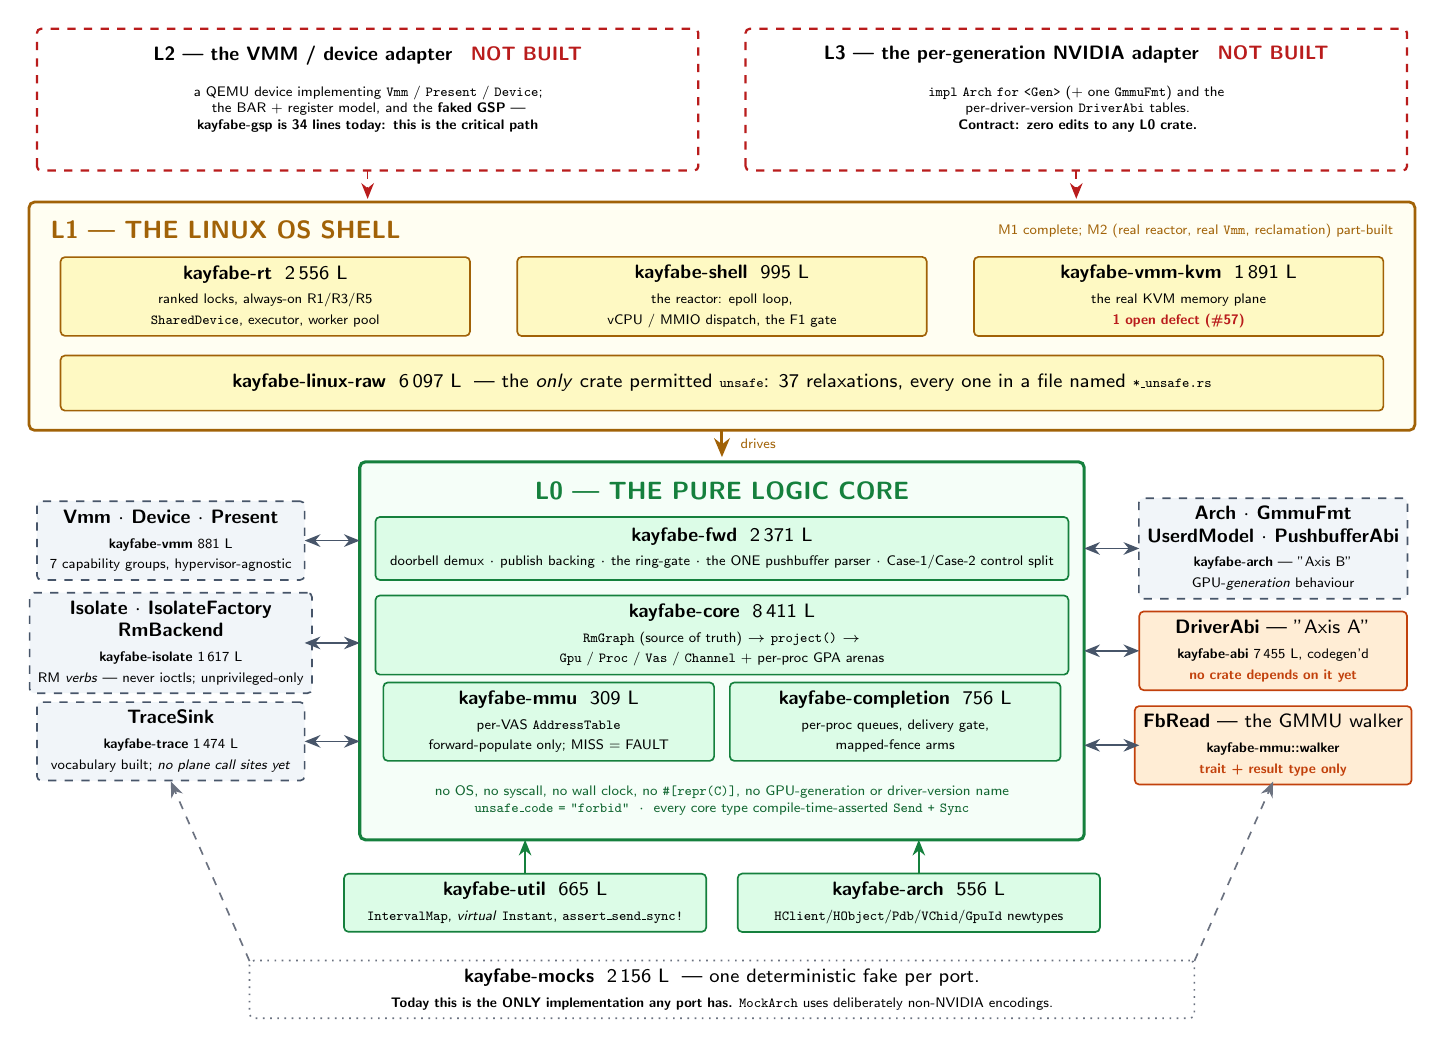
\begin{tikzpicture}[x=1mm,y=1mm, font=\sffamily\scriptsize]
\def\tc#1{{\ttfamily\fontsize{5.4}{6}\selectfont #1}}

% ============================================================== L2 and L3 ==
\draw[draw=kfhostln, dashed, line width=0.8pt, rounded corners=1.5pt, fill=white]
  (-87,99) rectangle (-3,117);
\node[align=center, anchor=north] at (-45,116)
  {\textbf{L2 — the VMM / device adapter}\;\; \unbuilt};
\node[align=center, anchor=north, font=\sffamily\tiny, text width=80mm] at (-45,111)
  {a QEMU device implementing \tc{Vmm} / \tc{Present} / \tc{Device};\\
   the BAR + register model, and the \textbf{faked GSP} —\\
   \textbf{kayfabe-gsp is 34 lines today: this is the critical path}};

\draw[draw=kfhostln, dashed, line width=0.8pt, rounded corners=1.5pt, fill=white]
  (3,99) rectangle (87,117);
\node[align=center, anchor=north] at (45,116)
  {\textbf{L3 — the per-generation NVIDIA adapter}\;\; \unbuilt};
\node[align=center, anchor=north, font=\sffamily\tiny, text width=80mm] at (45,111)
  {\tc{impl Arch for <Gen>} (+ one \tc{GmmuFmt}) and the\\
   per-driver-version \tc{DriverAbi} tables.\\
   \textbf{Contract: zero edits to any L0 crate.}};

\draw[ar, kfhostln, dashed] (-45,99) -- (-45,95.4);
\draw[ar, kfhostln, dashed] ( 45,99) -- ( 45,95.4);

% ================================================================ L1 band ==
\draw[draw=kfshellln, line width=1pt, rounded corners=2pt, fill=kfshell!22]
  (-88,66) rectangle (88,95);
\node[anchor=north west, font=\sffamily\bfseries\small, color=kfshellln]
  at (-86.5,93.8) {L1 — THE LINUX OS SHELL};
\node[anchor=north east, font=\sffamily\tiny, color=kfshellln]
  at (86.5,93.4) {M1 complete; M2 (real reactor, real \tc{Vmm}, reclamation) part-built};

\node[shellb, minimum width=52mm, minimum height=10mm] at (-58,83)
  {\textbf{kayfabe-rt} \;2\,556 L\\[1pt]\tiny ranked locks, always-on R1/R3/R5\\[-0.5pt]
   \tiny \tc{SharedDevice}, executor, worker pool};
\node[shellb, minimum width=52mm, minimum height=10mm] at (0,83)
  {\textbf{kayfabe-shell} \;995 L\\[1pt]\tiny the reactor: epoll loop,\\[-0.5pt]
   \tiny vCPU / MMIO dispatch, the F1 gate};
\node[shellb, minimum width=52mm, minimum height=10mm] at (58,83)
  {\textbf{kayfabe-vmm-kvm} \;1\,891 L\\[1pt]\tiny the real KVM memory plane\\[-0.5pt]
   \tiny \textbf{\color{kfhostln}1 open defect (\#57)}};
\node[shellb, minimum width=168mm, minimum height=7mm] at (0,72)
  {\textbf{kayfabe-linux-raw} \;6\,097 L \;— the \emph{only} crate permitted \tc{unsafe}:
   37 relaxations, every one in a file named \tc{*\_unsafe.rs}};

\draw[arw, kfshellln] (0,66) -- (0,62.6) node[midway, right=1mm, font=\sffamily\tiny, color=kfshellln]{drives};

% ================================================================ L0 band ==
\draw[draw=kfcoreln, line width=1.1pt, rounded corners=2pt, fill=kfcore!28]
  (-46,14) rectangle (46,62);
\node[anchor=north, font=\sffamily\bfseries\small, color=kfcoreln] at (0,60.6)
  {L0 — THE PURE LOGIC CORE};

\node[coreb, minimum width=88mm, minimum height=8mm] at (0,51)
  {\textbf{kayfabe-fwd} \;2\,371 L\\[1pt]
   \tiny doorbell demux $\cdot$ publish backing $\cdot$ the ring-gate $\cdot$ the ONE pushbuffer parser $\cdot$ Case-1/Case-2 control split};
\node[coreb, minimum width=88mm, minimum height=10mm] at (0,40)
  {\textbf{kayfabe-core} \;8\,411 L\\[1pt]
   \tiny \tc{RmGraph} (source of truth) $\rightarrow$ \tc{project()} $\rightarrow$\\[-0.5pt]
   \tiny \tc{Gpu} / \tc{Proc} / \tc{Vas} / \tc{Channel} + per-proc GPA arenas};
\node[coreb, minimum width=42mm, minimum height=8mm] at (-22,29)
  {\textbf{kayfabe-mmu} \;309 L\\[1pt]\tiny per-VAS \tc{AddressTable}\\[-0.5pt]\tiny forward-populate only; MISS = FAULT};
\node[coreb, minimum width=42mm, minimum height=8mm] at (22,29)
  {\textbf{kayfabe-completion} \;756 L\\[1pt]\tiny per-proc queues, delivery gate,\\[-0.5pt]\tiny mapped-fence arms};
\node[align=center, font=\sffamily\tiny, color=kfcoreln!80!black, text width=86mm] at (0,19)
  {no OS, no syscall, no wall clock, no \tc{\#[repr(C)]}, no GPU-generation or driver-version name\\
   \tc{unsafe\_code = "forbid"} \;$\cdot$\; every core type compile-time-asserted \tc{Send + Sync}};

% ============================================================ ports, left ==
\node[portb, minimum width=34mm, minimum height=10mm] at (-70,52)
  {\textbf{Vmm} $\cdot$ \textbf{Device} $\cdot$ \textbf{Present}\\[1pt]
   \tiny \textbf{kayfabe-vmm} 881 L\\[-0.5pt]\tiny 7 capability groups, hypervisor-agnostic};
\node[portb, minimum width=34mm, minimum height=11mm] at (-70,39)
  {\textbf{Isolate} $\cdot$ \textbf{IsolateFactory}\\ \textbf{RmBackend}\\[1pt]
   \tiny \textbf{kayfabe-isolate} 1\,617 L\\[-0.5pt]\tiny RM \emph{verbs} — never ioctls; unprivileged-only};
\node[portb, minimum width=34mm, minimum height=9mm] at (-70,26.5)
  {\textbf{TraceSink}\\[1pt]\tiny \textbf{kayfabe-trace} 1\,474 L\\[-0.5pt]
   \tiny vocabulary built; \emph{no plane call sites yet}};

\draw[arb, kfportln] (-53,52) -- (-46,52);
\draw[arb, kfportln] (-53,39) -- (-46,39);
\draw[arb, kfportln] (-53,26.5) -- (-46,26.5);

% =========================================================== ports, right ==
\node[portb, minimum width=34mm, minimum height=11mm] at (70,51)
  {\textbf{Arch} $\cdot$ \textbf{GmmuFmt}\\ \textbf{UserdModel} $\cdot$ \textbf{PushbufferAbi}\\[1pt]
   \tiny \textbf{kayfabe-arch} — "Axis B"\\[-0.5pt]\tiny GPU-\emph{generation} behaviour};
\node[stubb, minimum width=34mm, minimum height=10mm] at (70,38)
  {\textbf{DriverAbi} — "Axis A"\\[1pt]
   \tiny \textbf{kayfabe-abi} 7\,455 L, codegen'd\\[-0.5pt]
   \tiny \textbf{\color{kfstubln}no crate depends on it yet}};
\node[stubb, minimum width=34mm, minimum height=9mm] at (70,26)
  {\textbf{FbRead} — the GMMU walker\\[1pt]
   \tiny \textbf{kayfabe-mmu::walker}\\[-0.5pt]\tiny \textbf{\color{kfstubln}trait + result type only}};

\draw[arb, kfportln] (53,51) -- (46,51);
\draw[arb, kfportln] (53,38) -- (46,38);
\draw[arb, kfportln] (53,26) -- (46,26);

% ================================================== shared vocabulary base ==
\node[coreb, minimum width=46mm, minimum height=7mm] at (-25,6)
  {\textbf{kayfabe-util} \;665 L\\[1pt]\tiny \tc{IntervalMap}, \emph{virtual} \tc{Instant}, \tc{assert\_send\_sync!}};
\node[coreb, minimum width=46mm, minimum height=7mm] at (25,6)
  {\textbf{kayfabe-arch} \;556 L\\[1pt]\tiny \tc{HClient}/\tc{HObject}/\tc{Pdb}/\tc{VChid}/\tc{GpuId} newtypes};
\draw[ar, kfcoreln] (-25,9.6) -- (-25,14);
\draw[ar, kfcoreln] ( 25,9.6) -- ( 25,14);

\node[box, fill=white, draw=kfgrey, dotted, minimum width=120mm, minimum height=7mm] at (0,-5)
  {\textbf{kayfabe-mocks} \;2\,156 L \;— one deterministic fake per port.\\[1pt]
   \tiny \textbf{Today this is the ONLY implementation any port has.} \tc{MockArch} uses deliberately non-NVIDIA encodings.};
\draw[dashar, kfgrey] (-60,-1.4) -- (-70,21.4);
\draw[dashar, kfgrey] ( 60,-1.4) -- ( 70,21.4);

\end{tikzpicture}
}
\caption{The layer model and the hexagonal ports. Line counts are measured at \code{6ce8599}
(\code{crates/*/src/**/*.rs}; \code{kayfabe-abi}'s figure includes its detached offline
generator). Implementor census, counted from \code{impl <Trait> for} across the tree:
\code{FbRead} has \emph{no} implementation of any kind; \code{Device}, \code{Present},
\code{Arch}, \code{GspModel}, \code{Isolate}, \code{IsolateFactory} and \code{RmBackend} have
only mocks or test types; \code{Vmm} has one real adapter (\code{KvmVmm}); \code{TraceSink} has
two in-crate implementations. \code{kayfabe-gsp} joined the L0 band at this revision — it is a
pure logic crate and is covered by all four CI boundary greps — but the L2 shell that would call
it does not exist.}
\label{fig:layers}
\end{figure}\end{landscape}

\subsection{The crate dependency graph}

Figure~\ref{fig:deps} is derived from every \file{Cargo.toml} in the tree and cross-checked
against \file{Cargo.lock}; it is not drawn from the design documents. Three findings come
straight off it.

\textbf{The external dependency surface is essentially zero.} In the whole workspace there are
three external crates: \code{libc} — a real dependency of \code{kayfabe-linux-raw} only, and a
\emph{dev}-dependency of \code{kayfabe-vmm-kvm} and \code{tests} for asserting exact errnos —
plus \code{trybuild} and \code{proptest}, both dev-only. Thirteen of the sixteen crates have no
external dependency of any kind. Whatever else is true, the supply-chain surface is not a place
to look for problems.

\textbf{The graph is acyclic, including dev edges}, which the strictly lower-triangular shape of
the matrix demonstrates directly. \emph{The ordering that makes it lower-triangular had to change
at this revision:} \code{gsp} was a leaf sitting above \code{abi} and \code{trace}, and now
depends on both, so it moved below them. The re-ordering is the matrix's own record of the crate
ceasing to be a leaf.

\textbf{But the claimed strata are not disjoint, and the documents imply they are.}
\code{kayfabe-mmu} — a core crate — depends on the \code{kayfabe-isolate} \emph{port} (it needs
\code{HostHandle}). \code{kayfabe-core} and \code{kayfabe-fwd} depend on the \code{trace} and
\code{vmm} ports. \code{kayfabe-gsp} — also a core crate — depends on the \code{abi} and
\code{trace} ports. "Core" and "port" are one DAG with a purity rule, not two layers. That is a
defensible design (the trace crate had to sit \emph{below} core so every plane could emit into
it), but a reader who takes the hexagon picture literally will be surprised by the manifests.

\begin{claimbox}\small
\textbf{The previous revision of this paper called \code{kayfabe-abi} and \code{kayfabe-gsp}
"disconnected islands: nothing in the workspace — not \code{tests}, not \code{fuzz} — depends on
either". That was true then. Half of it is false now, and the surviving half is sharper.}

\smallskip
\emph{Re-checked against the manifests and the source, not inherited.} \code{kayfabe-abi} is no
longer an island: \file{crates/kayfabe-gsp/Cargo.toml} lists it, and five of the eight
\code{kayfabe-gsp} modules use it (\code{lib}, \code{boot}, \code{element}, \code{fault},
\code{replay}) — it supplies the RPC envelope view and the version-keyed layout values. So the
7\,455 lines of oracle-tested wire decoding finally have a consumer, and that consumer is the one
the crate was written for.

\smallskip
\code{kayfabe-gsp} \textbf{is still an island in the direction that matters}: the only manifest
that lists it is \file{tests/Cargo.toml}. No production crate depends on it, nothing constructs
its inputs outside \code{tests/}, and its output type \code{RpcCommand} has \textbf{zero}
references anywhere in the tree outside the crate that defines it. It is 3\,550 lines of working
protocol logic with a test suite and no caller — which is exactly as interesting as the old
caption said, one level up the stack.
\end{claimbox}

\begin{landscape}\begin{figure}[p]
\centering
\adjustbox{max width=\linewidth, max totalheight=0.86\textheight}{% ===========================================================================
% FIGURE — the crate dependency graph, DERIVED from every Cargo.toml in the
% workspace (root, crates/*/Cargo.toml, crates/kayfabe-abi/gen, tests/, fuzz/)
% and cross-checked against Cargo.lock, at b612a91. Rows = the depending
% crate, columns = the crate depended on. Crates are listed in topological
% order, so the matrix being strictly lower-triangular IS the proof that the
% graph is acyclic.
%
% ★ The edge list was RE-DERIVED BY SCRIPT at this revision, not edited from
% the previous one. Two changes fell out that nobody was looking for:
%   - `rmrpc` is new (row/col 13) and must sit BELOW both `gsp` and `core`;
%   - `mocks` acquired an `abi` edge (2dac655 promoted WireClassArch into it).
% ===========================================================================
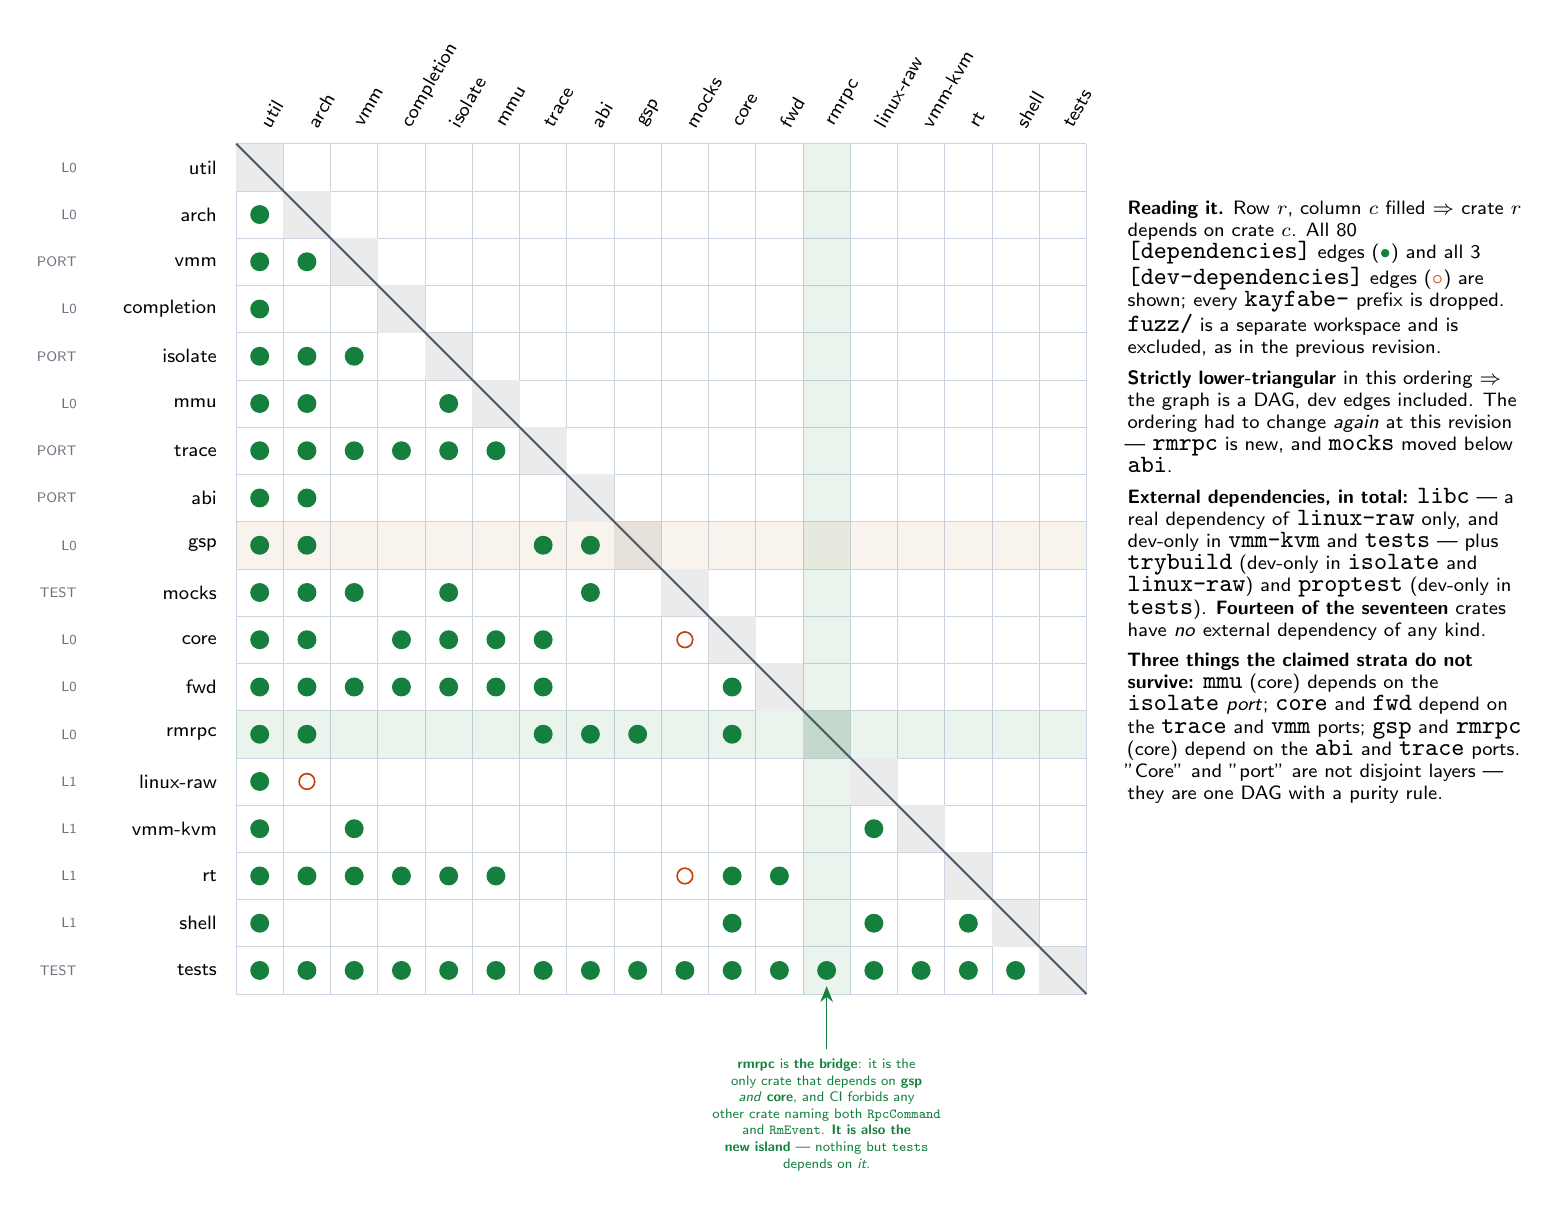
\begin{tikzpicture}[x=1mm,y=1mm, font=\sffamily\scriptsize]
\def\cs{6}        % cell size (mm)
\def\N{18}

% -- crate list in topological order -----------------------------------------
\def\crates{
  1/util/L0,
  2/arch/L0,
  3/vmm/PORT,
  4/completion/L0,
  5/isolate/PORT,
  6/mmu/L0,
  7/trace/PORT,
  8/abi/PORT,
  9/gsp/L0,
  10/mocks/TEST,
  11/core/L0,
  12/fwd/L0,
  13/rmrpc/L0,
  14/linux-raw/L1,
  15/vmm-kvm/L1,
  16/rt/L1,
  17/shell/L1,
  18/tests/TEST}

% -- grid --------------------------------------------------------------------
\foreach \i in {0,...,\N}{
  \draw[kfrule, line width=0.25pt] (0,-\i*\cs) -- (\N*\cs,-\i*\cs);
  \draw[kfrule, line width=0.25pt] (\i*\cs,0) -- (\i*\cs,-\N*\cs);
}
% diagonal band (a crate never depends on itself)
\foreach \i in {1,...,\N}{
  \fill[black!8] ({(\i-1)*\cs},{-(\i-1)*\cs}) rectangle ({\i*\cs},{-\i*\cs});
}
\draw[kfportln, line width=0.7pt] (0,0) -- (\N*\cs,-\N*\cs);

% -- highlight the rmrpc row + column (the new bridge, and the new island) ----
\fill[kfcoreln, opacity=0.09] (0,{-12*\cs}) rectangle ({\N*\cs},{-13*\cs});
\fill[kfcoreln, opacity=0.09] ({12*\cs},0) rectangle ({13*\cs},{-\N*\cs});
% -- and the gsp row, faintly: it is no longer the island -------------------
\fill[kfshellln, opacity=0.07] (0,{-8*\cs}) rectangle ({\N*\cs},{-9*\cs});

% -- row labels (left) -------------------------------------------------------
\foreach \i/\n/\g in \crates {
  \node[anchor=east, font=\sffamily\scriptsize] at (-1.2,{-(\i-0.5)*\cs}) {\n};
  \node[anchor=east, font=\sffamily\tiny, color=kfgrey] at (-19,{-(\i-0.5)*\cs}) {\g};
}
% -- column labels (top, rotated) --------------------------------------------
\foreach \i/\n/\g in \crates {
  \node[anchor=west, rotate=60, font=\sffamily\scriptsize] at ({(\i-0.5)*\cs},1.2) {\n};
}

% -- the edges ---------------------------------------------------------------
% \dep{row}{col}  = [dependencies]        \dev{row}{col} = [dev-dependencies]
\def\dep#1#2{\node[circle, fill=kfcoreln, inner sep=0.85mm]
   at ({(#2-0.5)*\cs},{-(#1-0.5)*\cs}) {};}
\def\dev#1#2{\node[circle, draw=kfstubln, line width=0.6pt, inner sep=0.7mm]
   at ({(#2-0.5)*\cs},{-(#1-0.5)*\cs}) {};}

\dep{2}{1}
\dep{3}{1}\dep{3}{2}
\dep{4}{1}
\dep{5}{1}\dep{5}{2}\dep{5}{3}
\dep{6}{1}\dep{6}{2}\dep{6}{5}
\dep{7}{1}\dep{7}{2}\dep{7}{3}\dep{7}{4}\dep{7}{5}\dep{7}{6}
\dep{8}{1}\dep{8}{2}
\dep{9}{1}\dep{9}{2}\dep{9}{7}\dep{9}{8}
\dep{10}{1}\dep{10}{2}\dep{10}{3}\dep{10}{5}\dep{10}{8}
\dep{11}{1}\dep{11}{2}\dep{11}{4}\dep{11}{5}\dep{11}{6}\dep{11}{7}\dev{11}{10}
\dep{12}{1}\dep{12}{2}\dep{12}{3}\dep{12}{4}\dep{12}{5}\dep{12}{6}\dep{12}{7}\dep{12}{11}
\dep{13}{1}\dep{13}{2}\dep{13}{7}\dep{13}{8}\dep{13}{9}\dep{13}{11}
\dep{14}{1}\dev{14}{2}
\dep{15}{1}\dep{15}{3}\dep{15}{14}
\dep{16}{1}\dep{16}{2}\dep{16}{3}\dep{16}{4}\dep{16}{5}\dep{16}{6}\dev{16}{10}\dep{16}{11}\dep{16}{12}
\dep{17}{1}\dep{17}{11}\dep{17}{14}\dep{17}{16}
\dep{18}{1}\dep{18}{2}\dep{18}{3}\dep{18}{4}\dep{18}{5}\dep{18}{6}\dep{18}{7}\dep{18}{8}
\dep{18}{9}\dep{18}{10}\dep{18}{11}\dep{18}{12}\dep{18}{13}\dep{18}{14}\dep{18}{15}
\dep{18}{16}\dep{18}{17}

% -- annotations -------------------------------------------------------------
\draw[ar, kfcoreln] ({12.5*\cs},{-\N*\cs-7}) -- ({12.5*\cs},{-\N*\cs+1});
\node[anchor=north, font=\sffamily\tiny, color=kfcoreln, align=center]
  at ({12.5*\cs},{-\N*\cs-7})
  {\textbf{rmrpc} is \textbf{the bridge}: it is the\\ only crate that depends on
   \textbf{gsp}\\ \emph{and} \textbf{core}, and CI forbids any\\ other crate naming both
   {\ttfamily RpcCommand}\\ and {\ttfamily RmEvent}. \textbf{It is also the}\\
   \textbf{new island} — nothing but {\ttfamily tests}\\ depends on \emph{it}.};

\node[anchor=north west, font=\sffamily\scriptsize, align=left]
  at ({\N*\cs+4},{-1*\cs}) {%
  \begin{minipage}{50mm}\raggedright\scriptsize
  \textbf{Reading it.} Row $r$, column $c$ filled $\Rightarrow$ crate $r$ depends on
  crate $c$. All 80 \code{[dependencies]} edges ({\color{kfcoreln}$\bullet$}) and all
  3 \code{[dev-dependencies]} edges ({\color{kfstubln}$\circ$}) are shown; every
  \code{kayfabe-} prefix is dropped. \code{fuzz/} is a separate workspace and is
  excluded, as in the previous revision.\\[3pt]
  \textbf{Strictly lower-triangular} in this ordering $\Rightarrow$ the graph is a DAG,
  dev edges included. The ordering had to change \emph{again} at this revision —
  \code{rmrpc} is new, and \code{mocks} moved below \code{abi}.\\[3pt]
  \textbf{External dependencies, in total:} \code{libc} — a real dependency of
  \code{linux-raw} only, and dev-only in \code{vmm-kvm} and \code{tests} — plus
  \code{trybuild} (dev-only in \code{isolate} and \code{linux-raw}) and \code{proptest}
  (dev-only in \code{tests}). \textbf{Fourteen of the seventeen} crates have \emph{no}
  external dependency of any kind.\\[3pt]
  \textbf{Three things the claimed strata do not survive:} \code{mmu} (core) depends on
  the \code{isolate} \emph{port}; \code{core} and \code{fwd} depend on the
  \code{trace} and \code{vmm} ports; \code{gsp} and \code{rmrpc} (core) depend on the
  \code{abi} and \code{trace} ports. "Core" and "port" are not disjoint
  layers — they are one DAG with a purity rule.
  \end{minipage}};

\end{tikzpicture}
}
\caption{The crate dependency matrix, derived from the manifests at \code{6ce8599}.
\code{kayfabe-abi} is no longer an island — \code{kayfabe-gsp} consumes it, which is what it was
written for. \code{kayfabe-gsp} still is one: the only manifest that names it is
\file{tests/Cargo.toml}, so 3\,550 lines of protocol logic have a test suite and \emph{no
production caller}. Note also that the previous revision's matrix omitted one real edge,
\code{tests}\,$\rightarrow$\,\code{rt}; it showed 65 dependency edges where the manifests had 66.}
\label{fig:deps}
\end{figure}\end{landscape}

\subsection{The data path}

Figure~\ref{fig:datapath} traces one guest GPU operation from a CUDA call to real silicon and
back, naming the symbol each step lives at. Three things about it are worth stating in prose.

\textbf{The plan/execute/commit shape is the whole concurrency design.} A host RM verb can block
for a long time — the host RM serializes every ioctl per client, and it waits
\emph{uninterruptibly}, so one wedged verb parks every isolate that shares the client in
D-state. Invariant \textbf{R1} therefore forbids issuing a verb while any ranked lock is held.
That forces a three-phase shape: \emph{plan} under locks, \emph{execute} with no lock held,
\emph{commit} after re-acquiring. And because the locks were dropped in the middle, invariant
\textbf{R5} requires the commit to re-validate everything the plan assumed. This is not free —
\S\ref{sec:discussion} covers what it costs.

\textbf{The ring gate is the \#14 fix, and it is now structural in the type system.} Before any
host operation, a doorbell submission's entire working set must already be published into
\emph{this} \code{Vas}'s own host address space. If it is not, the call refuses with
\code{NoVas} having issued zero host operations. The failure it prevents is exactly the one the C
artifact hit on real hardware: the losing process's identical guest VAs were never published into
its own host GR address space, so the host GPU faulted past the shared prefix. At the previous pin
this was a call-graph property — "every path happens to go through \code{plan\_doorbell}". At
\code{634b253} it stopped being one: \code{VerbPlan::Doorbell} is \code{\#[non\_exhaustive]}, so no
struct expression for it exists outside \code{kayfabe-isolate}, and the sole constructor
\code{VerbPlan::gated\_doorbell} \emph{runs} the gate. Constructing an ungated doorbell is now
compile error E0639, pinned by a \code{trybuild} row (\file{crates/kayfabe-isolate/tests/ui/}).

\textbf{The upper half of the diagram is half-built, and the half that is missing moved.} At the
previous pin there was no register model, no GSP message-queue transport and no RPC decode. All
three now exist, in \code{kayfabe-gsp}. What still does not exist is (a) any adapter that
implements \code{GuestRam} or \code{Device} outside \code{tests/}, and (b) the bridge from the
GSP's decoded output to the core's input — \code{RpcCommand} has zero references anywhere in the
tree outside the crate that defines it. So the headline sentence survives verbatim:
\textbf{nothing in the repository produces an \code{RmEvent} from real guest bytes}, and the
core's control-plane input is still synthesised by the test suite. \S\ref{sec:gsp} is about what
changed underneath that sentence.

\begin{landscape}\begin{figure}[p]
\centering
\adjustbox{max width=\linewidth, max totalheight=0.86\textheight}{% ===========================================================================
% FIGURE — the data path, verified function-by-function against the tree at
% 0b78102.  Every box carries the file it lives in.  The dashed red band is
% the part that does not exist.
% ===========================================================================
\begin{tikzpicture}[x=1mm,y=1mm, font=\sffamily\scriptsize]
\def\tc#1{{\ttfamily\fontsize{5.4}{6}\selectfont #1}}
\def\fl#1{{\fontsize{5}{5.6}\selectfont\color{kfgrey} #1}}

% ------------------------------------------------------------------ lanes --
\foreach \t/\b/\c/\n in {
   100/88/kfguest/{GUEST\\(unmodified)},
    84/70/kfemul/{EMULATED GPU\\+ FAKED GSP},
    66/50/kfshell/{L1 — THE\\OS SHELL},
    46/12/kfcore/{L0 — THE\\PURE CORE},
     8/-6/kfport/{ISOLATE\\(unprivileged)},
   -10/-24/kfhost/{HOST KERNEL\\+ REAL GPU}}
{
  \fill[\c!35, rounded corners=1.5pt] (-86,\b) rectangle (92,\t);
  \node[rotate=90, font=\sffamily\bfseries\tiny, color=black!62, align=center]
     at (-89.5,{(\t+\b)/2}) {\n};
}

% =============================================== GUEST =====================
\node[guestb, minimum width=54mm, minimum height=7mm] (app) at (-55,94)
  {CUDA / Vulkan application\\[1pt]\tiny \tc{cuMemAlloc}, \tc{cuLaunchKernel}, \tc{cuStreamSynchronize}};
\node[guestb, minimum width=76mm, minimum height=7mm] (gdrv) at (35,94)
  {\textbf{stock NVIDIA kernel driver} — unmodified, unaware it is virtualised\\[1pt]
   \tiny RM object allocs $\rightarrow$ GSP RPC ring writes $\cdot$ GPU page-table builds $\cdot$ MMIO doorbell stores};
\draw[ar] (app) -- (gdrv);

% =============================================== EMULATED DEVICE ===========
\node[box, fill=white, draw=kfhostln, dashed, line width=0.8pt,
      minimum width=104mm, minimum height=12mm] (l2) at (-30,77)
  {\textbf{\color{kfhostln}THIS LANE IS UNBUILT.}\; The BAR/register model, the GSP\\
   message-queue transport, the RPC decode.\\[1.5pt]
   \tiny \tc{kayfabe-gsp} = 34 lines (a 3-variant \tc{BootPhase} enum that nothing references).\\[-0.5pt]
   \tiny \tc{kayfabe-abi} \emph{is} built — 7\,455 lines of codegen'd wire tables — but \textbf{no crate depends on it}.\\[-0.5pt]
   \tiny \textbf{So nothing here produces an \tc{RmEvent} from real guest bytes yet.}};
\node[box, fill=white, draw=kfhostln, dashed, minimum width=58mm, minimum height=9mm] (bar) at (52,77)
  {doorbell BAR decode: offset $\rightarrow$ \tc{(GpuId, token)}\\[1pt]
   \tiny only implementor in the tree is the test device\\[-0.5pt]\fl{tests/src/guest.rs:185}};

\draw[ar, kfhostln, dashed] (-70,88) -- (-70,83.2)
  node[midway, left=0.8mm, align=center, font=\sffamily\tiny, color=kfhostln]{RM ioctls,\\GSP RPC};
\draw[ar, kfguestln, line width=1pt] (52,88) -- (52,81.6)
  node[midway, right=0.8mm, font=\sffamily\tiny, color=kfguestln]{MMIO store};

% =============================================== L1 SHELL ==================
\node[shellb, minimum width=50mm, minimum height=11mm] (vcpu) at (-58,58)
  {\textbf{1}\; \tc{KvmVcpu::run} $\rightarrow$ \tc{VcpuExit::Mmio}\\[1pt]
   \fl{linux-raw/src/vcpu\_unsafe.rs:433}\\[2pt]
   \textbf{2}\; \tc{VcpuRunner::dispatch} / \tc{classify\_exit}\\[1pt]
   \fl{vmm-kvm/src/vcpu.rs:266, :329}};
\node[shellb, minimum width=44mm, minimum height=11mm] (dev) at (-3,58)
  {\textbf{3}\; \tc{dyn Device::mmio\_write}\\[1pt]\fl{kayfabe-vmm/src/lib.rs:849}\\[2pt]
   {\color{kfhostln}\textbf{no production implementor exists}}};
\node[shellb, minimum width=52mm, minimum height=11mm] (sd) at (52,58)
  {\textbf{4}\; \tc{SharedDevice::doorbell} $\rightarrow$ \tc{verb\_op}\\[1pt]
   \fl{kayfabe-rt/src/device.rs:1180, :1035}\\[2pt]
   \tiny ranked locks — rank 0 device \tc{RwLock},\\[-0.5pt]\tiny rank 1 per-\tc{Proc} \tc{Mutex}};
\draw[ar] (bar.south) -- (52,63.6);
\draw[ar] (dev) -- (sd);
\draw[ar] (vcpu) -- (dev);

% =============================================== L0 CORE ===================
\node[coreb, minimum width=76mm, minimum height=13mm] (ctl) at (-45,38)
  {\textbf{C}\; the CONTROL plane — \tc{Gpu::apply(RmEvent)}\\[1pt]
   \fl{core/src/gpu.rs:2738 $\rightarrow$ Spine::apply :1202 — snapshot, then rollback on any fault}\\[2pt]
   \tiny \tc{RmGraph::apply} $\rightarrow$ \tc{project()} $\rightarrow$ \tc{refresh} $\rightarrow$ \tc{sync\_rpc\_mappings}
     $\rightarrow$ \tc{AddressTable::bind}\\[-0.5pt]
   \tiny \textbf{forward-populate only} — the table is written from declared protocol facts\\[-0.5pt]
   \tiny and never reverse-resolved out of guest memory; a lookup miss is a fault};
\node[coreb, minimum width=88mm, minimum height=9mm] (route) at (44,40)
  {\textbf{5}\; \tc{route\_doorbell} — token $\rightarrow$ \tc{vChid} $\rightarrow$ \tc{(GpuId,VChid)} $\rightarrow$ \tc{(ProcId,ChanId)}\\[1pt]
   \fl{kayfabe-fwd/src/lib.rs:1052} \;— a pure projection lookup; an unknown token is a loud fault};
\node[box, fill=kfcore, draw=kfcoreln, line width=1.3pt,
      minimum width=88mm, minimum height=11mm] (gate) at (44,27)
  {\textbf{6}\; \tc{plan\_doorbell} — \textbf{★ THE \#14 RING GATE}\\[1pt]
   \fl{kayfabe-fwd/src/lib.rs:1140; the gate itself at :1162--1175}\\[2pt]
   \tiny every VA in the submission's working set must already be published into \emph{this}\\[-0.5pt]
   \tiny \tc{Vas}'s own host address space, or the call refuses \tc{NoVas} having issued zero host operations};
\node[box, fill=white, draw=kfcoreln, minimum width=76mm, minimum height=11mm] (r5) at (-45,20)
  {\textbf{7b}\; \tc{commit\_phase} — \textbf{★ invariant R5}\\[1pt]
   \fl{rt/device.rs:777 $\rightarrow$ fwd::commit\_doorbell :1219}\\[2pt]
   \tiny the locks were dropped for step 7, so everything the plan assumed is
   \textbf{re-validated}\\[-0.5pt]
   \tiny before any state changes; a refusal hands back its orphans.
   Bounded re-plan: \tc{MAX\_COMMIT\_RETRIES = 8}};
\draw[ar] (sd.south) -- (52,44.6);
\draw[ar] (route) -- (gate);

% =============================================== ISOLATE ===================
\node[portb, minimum width=104mm, minimum height=12mm, fill=white] (worker) at (32,1)
  {\textbf{7}\; \tc{Worker::execute(\&VerbPlan)} — \textbf{★ NO LOCK IS HELD HERE (invariant R1)}\\[1pt]
   \fl{kayfabe-isolate/src/lib.rs:1096; the assertion at :1097}\\[2pt]
   \tiny \tc{alloc\_vaspace} $\cdot$ \tc{alloc\_sysmem} $\cdot$ \tc{map\_gpu\_va} $\cdot$ \tc{alloc\_channel(vas,\,engine)}
   $\cdot$ \tc{alloc\_engine\_object}\\[-0.5pt]
   \tiny $\cdot$ \tc{schedule} $\cdot$ \tc{control} $\cdot$ \tc{ring\_doorbell} $\cdot$ \tc{free} $\cdot$ \tc{unmap\_gpu\_va}
   $\cdot$ \tc{export\_surface} — 12 verbs, all unprivileged};
\node[portb, minimum width=62mm, minimum height=10mm, fill=white] (poolgate) at (-52,1)
  {one isolate process per \textbf{(guest process, GPU)} pair\\[1pt]
   \tiny a bounded pool of single-in-flight workers (default 4)\\[-0.5pt]
   \tiny \textbf{\color{kfhostln}the only \tc{RmBackend} implementation today is the mock}};
\draw[ar, line width=1.1pt] (gate.south) -- (44,7.2);
\draw[ar, dashed] (worker.north west) -- (r5.south east);

% =============================================== HOST ======================
\node[hostb, minimum width=72mm, minimum height=10mm] (rm) at (-38,-17)
  {\textbf{8}\; real \tc{ioctl}s on \tc{/dev/nvidiactl} and \tc{/dev/nvidia0}\\[1pt]
   \tiny issued by an ordinary unprivileged uid inside a sandbox, so the host's own\\[-0.5pt]
   \tiny kernel RM legitimately re-derives every privileged step for itself};
\node[hostb, minimum width=64mm, minimum height=10mm] (gpu) at (48,-17)
  {\textbf{9}\; \textbf{the real GPU executes the guest's own pushbuffer}\\[1pt]
   \tiny no engine is ever emulated — GR's golden context is produced by\\[-0.5pt]
   \tiny FECS/GPCCS microcode on silicon and is a hard boundary};
\draw[ar] (0,-5.2) -- (0,-12);
\draw[ar] (rm) -- (gpu);

% =============================================== RETURN PATH ===============
\node[box, fill=kfshell, draw=kfshellln, minimum width=178mm, minimum height=11mm] at (3,-34)
  {\textbf{The completion path back — different threads, same tree}\\[2pt]
   \textbf{10} host readiness fd $\rightarrow$ \tc{Poller::wait} \fl{(linux-raw/epoll\_unsafe.rs:189)} $\rightarrow$
   \tc{Reactor::run\_with} \fl{(shell/reactor.rs:303)} $\rightarrow$ \tc{Registrar::resolve}
   $\rightarrow$ inbox \tc{CoreEvent::SourceSignal}\\[1.5pt]
   \textbf{11} \tc{Executor::drain\_one} \fl{(rt/executor.rs:74)} $\rightarrow$
   \tc{SharedDevice::signal\_source} \fl{(rt/device.rs:1423)} $\rightarrow$
   \tc{SourceRegistry::dispatch} $\rightarrow$ \textbf{the owning proc's own} \tc{CompletionQueue}\\[1.5pt]
   \textbf{12} \tc{deliver\_completions} / \tc{poll\_completions} \fl{(fwd/lib.rs:1346, :1359)}
   $\rightarrow$ \tc{Vmm::raise\_irq(IrqSpec::Msix(0))} $\rightarrow$ the guest's own interrupt handler};
\draw[ar, kfhostln, line width=1pt] (84,-12) -- (88,-12) -- (88,-28.5);

\end{tikzpicture}
}
\caption{The data path, verified function by function against the tree at \code{6ce8599}.
Numbered steps are the execution plane; \textbf{C} is the control plane, which populates the
address table from declared protocol facts. Boxes name \emph{symbols}, not line numbers: the
repository converted its own 105 pins to symbols in \code{3fd1455} after they drifted, and six of
this figure's pins had drifted by this revision. Red text marks what does not exist.}
\label{fig:datapath}
\end{figure}\end{landscape}

\subsection{The isolation model}

\begin{landscape}\begin{figure}[p]
\centering
\adjustbox{max width=\linewidth, max totalheight=0.86\textheight}{% ===========================================================================
% FIGURE — the process / isolation model, and the problem it exists to solve.
% Verified against kayfabe-core/src/gpu.rs (Proc, Vas, Channel, IsolateBox),
% gpa.rs (GpaSpace/GpaArena), kayfabe-isolate/src/lib.rs (IsolateFactory).
% ===========================================================================
\begin{tikzpicture}[x=1mm,y=1mm, font=\sffamily\scriptsize]
\def\tc#1{{\ttfamily\fontsize{5.4}{6}\selectfont #1}}

% ---------------------------------------------------------------- the guest --
\node[guestb, minimum width=54mm, minimum height=14mm] (pa) at (-48,89)
  {\textbf{guest process A} \;(e.g.\ PyTorch)\\[2pt]
   \tiny \tc{hClient = 0xc1d00001}\\[-0.5pt]
   \tiny buffer at guest VA \tc{0x7f\_0000\_0000}\\[-0.5pt]
   \tiny channel handle \tc{0x00000010}};
\node[guestb, minimum width=54mm, minimum height=14mm] (pb) at (48,89)
  {\textbf{guest process B} \;(e.g.\ llama.cpp)\\[2pt]
   \tiny \tc{hClient = 0xc1d00001} \;\textbf{— the same value}\\[-0.5pt]
   \tiny buffer at guest VA \tc{0x7f\_0000\_0000} \;\textbf{— the same VA}\\[-0.5pt]
   \tiny channel handle \tc{0x00000010} \;\textbf{— the same handle}};
\node[align=center, font=\sffamily\tiny, color=kfhostln, text width=32mm] at (0,89)
  {\textbf{Not a corner case.}\\ Handles and guest VAs are\\ \emph{per-process namespaces};
   two\\ processes colliding on every\\ value is normal.\\[1.5pt]
   \textbf{This is bug \#14.}};

\draw[ar, kfguestln] (pa.south) -- ++(0,-4);
\draw[ar, kfguestln] (pb.south) -- ++(0,-4);

% --------------------------------------------------- what disambiguates them --
\node[emulb, minimum width=134mm, minimum height=10mm] at (0,74)
  {\textbf{The only values that are NOT process-chosen are the ones the guest \emph{kernel} assigns from real hardware:}\\[2pt]
   \tiny \tc{Pdb} — the page-directory base, which the GMMU itself keys page tables by
     $\Rightarrow$ \textbf{the memory boundary}\\[-0.5pt]
   \tiny \tc{VChid} — the virtual channel id a doorbell token decodes to
     $\Rightarrow$ \textbf{the execution boundary}\\[-0.5pt]
   \tiny Everything is keyed \tc{(GpuId, Pdb)} or \tc{(GpuId, VChid)}. Never on a client handle.
     Never on host CPU state — no CR3 is read anywhere.};

% ------------------------------------------------------------- the two Procs --
\foreach \x/\lbl/\pdb/\ch/\ar in {-46/A/0x0a1000/14/{[0x0000\_0000,\;0x1000\_0000)},
                                   46/B/0x0b7000/15/{[0x1000\_0000,\;0x2000\_0000)}}
{
  \draw[draw=kfcoreln, line width=1pt, rounded corners=2pt, fill=kfcore!30]
    (\x-31,11) rectangle (\x+31,65);
  \node[anchor=north, font=\sffamily\bfseries\small, color=kfcoreln] at (\x,64)
    {\tc{Proc} \lbl\; — one guest process};
  \node[coreb, minimum width=58mm, minimum height=10mm] at (\x,53)
    {\textbf{address plane}\\[1pt]
     \tiny \tc{Vas} per \tc{(GpuId, Pdb=\pdb)} — its own \tc{AddressTable}\\[-0.5pt]
     \tiny \textbf{and its own host address space} (the \#14 fix)};
  \node[coreb, minimum width=58mm, minimum height=10mm] at (\x,41)
    {\textbf{execution plane}\\[1pt]
     \tiny \tc{Channel} per \tc{vChid = \ch} + a per-proc \tc{ExecPlane}\\[-0.5pt]
     \tiny nothing scheduled is one-shot or device-global (the \#12 fix)};
  \node[coreb, minimum width=58mm, minimum height=10mm] at (\x,29)
    {\textbf{completion plane}\\[1pt]
     \tiny its own \tc{CompletionQueue} + \tc{FenceArms}; re-delivery is\\[-0.5pt]
     \tiny driven off \emph{this} proc's own poll (the starvation fix)};
  \node[coreb, minimum width=58mm, minimum height=10mm] at (\x,17)
    {\textbf{isolate + GPA arena}\\[1pt]
     \tiny a disjoint slice of the guest-physical window: \tc{\ar}\\[-0.5pt]
     \tiny \tc{GpaSpace::release} takes the arena \textbf{by value}};
}
\draw[arb, kfhostln, dashed, line width=0.8pt] (-16,41) -- (16,41);
\node[align=center, font=\sffamily\tiny, color=kfhostln, text width=30mm] at (0,35)
  {\textbf{no shared state}\\ on any of the\\ four planes};

% ------------------------------------------------------------- the isolates --
\node[portb, fill=white, minimum width=58mm, minimum height=11mm] (ia) at (-48,4)
  {\textbf{isolate process} for \tc{(Proc A, GPU 0)}\\[1pt]
   \tiny separate OS process, unprivileged uid, namespaces,\\[-0.5pt]
   \tiny \tc{pivot\_root}, seccomp, cleared env and fds\\[-0.5pt]
   \tiny a bounded pool of single-in-flight workers};
\node[portb, fill=white, minimum width=58mm, minimum height=11mm] (ib) at (48,4)
  {\textbf{isolate process} for \tc{(Proc B, GPU 0)}\\[1pt]
   \tiny its own host RM client; handles minted here are\\[-0.5pt]
   \tiny typed to \emph{this} isolate, so a cross-isolate handle\\[-0.5pt]
   \tiny does not merely fail — it does not type-check};
\draw[ar, kfcoreln] (-48,11) -- (ia.north);
\draw[ar, kfcoreln] ( 48,11) -- (ib.north);

\node[align=center, font=\sffamily\tiny, color=kfhostln, text width=32mm] at (0,4)
  {\textbf{Blast radius.} A guest process that\\ crashes, wedges or attacks its own\\ isolate loses that isolate
   and nothing\\ else. The claim is \textbf{process-grade},\\ not VM-grade, isolation between\\ guest processes.};

% -------------------------------------------------------------- the host GPU --
\node[hostb, minimum width=134mm, minimum height=10mm] (hg) at (0,-13)
  {\textbf{one real host GPU}, driven by the ordinary NVIDIA driver through ordinary unprivileged \tc{ioctl}s\\[2pt]
   \tiny the host's own kernel RM keeps the two isolates' address spaces, channels and contexts apart —
   we are not asking it for anything unusual};
\draw[ar] (ia.south) -- (ia.south |- hg.north);
\draw[ar] (ib.south) -- (ib.south |- hg.north);

% ---------------------------------------------------------------- honesty box --
\node[box, fill=kfhost!30, draw=kfhostln, minimum width=178mm, minimum height=11mm] at (0,-29)
  {\textbf{\color{kfhostln}What is actually running, as of this document (2026-08-20).}\\[2pt]
   \tiny The per-\tc{Proc} plane ownership above is \textbf{built, heavily tested against mocks, and
   now driven on real hardware} — \tc{kayfabe-isolate-host} is a real sandboxed, capability-less,\\[-0.5pt]
   \tiny six-namespace child holding \file{/dev/nvidiactl} and \file{/dev/nvidia0}, and it is what
   executes the guest's compute. Its \tc{RmBackend} issues real host RM ioctls.\\[-0.5pt]
   \tiny ★★★ \textbf{The multi-\tc{Proc} axis this figure exists to argue has been driven}: two
   CONCURRENT guest CUDA processes both computed (w299, 2026-08-14) — 3 isolates materialized,
   3 live, 0 refusing, distinct \tc{proc=} ids —\\[-0.5pt]
   \tiny and the C artifact's \#14 hang did NOT reproduce, even with the second started while the
   first was inside \tc{cuCtxCreate}. \textbf{\color{kfhostln}⊘ Two identical short workloads,
   emulated CE work, one VM.}\\[-0.5pt]
   \tiny \textbf{\color{kfhostln}A second context SEQUENTIALLY in one boot still hangs}, and
   \textbf{\color{kfhostln}there is no tenant axis at all} — no \tc{VmId} anywhere in
   \file{crates/}; cross-VM separation is incidental to two host processes.};

\end{tikzpicture}
}
\caption{The process and isolation model, and the problem it exists to solve. The per-\code{Proc}
ownership of all four planes is built and heavily tested against mocks; the sandboxed isolate
process at the bottom has never been spawned by this codebase.}
\label{fig:isolation}
\end{figure}\end{landscape}

The rule that generates the whole model is one sentence: \textbf{a guest process is a grouping
label, and it is never what an address or execution operation keys on.} Address operations key
on \code{(GpuId, Pdb)}; execution operations key on \code{(GpuId, VChid)}. \code{Proc} exists
only to own the isolate, the GPA arena and the lifecycle.

\code{Proc} membership is itself a \textbf{pure projection} of the RM graph — the
dup-connected components of declared user clients — never inferred from timing, never from
arrival order. That matters because it means two identical event streams delivered in different
orders produce bit-identical process boundaries, which is a property the test suite checks
directly by permuting streams.

\subsection{The lifecycle}

\begin{landscape}\begin{figure}[p]
\centering
\adjustbox{max width=\linewidth, max totalheight=0.86\textheight}{% ===========================================================================
% FIGURE — the lifecycle: the eight teardown triggers and the retire/reap
% split.  Source: docs/design/l1_os_shell.md §7.6 (T0..T7) and §7.8 (the
% conservation ledger), cross-checked against kayfabe-core/src/gpu.rs
% (Proc::retire, Gpu::reap_retired) and kayfabe-isolate (two-stage retire).
% Status colours are this document's reading of the tree, not the doc's.
% ===========================================================================
\begin{tikzpicture}[x=1mm,y=1mm, font=\sffamily\scriptsize]
\def\tc#1{{\ttfamily\fontsize{5.4}{6}\selectfont #1}}

% --------------------------------------------------------- the central law --
\node[box, fill=kfcore, draw=kfcoreln, line width=1.1pt,
      minimum width=176mm, minimum height=11mm] at (0,72)
  {\textbf{The law every path obeys: RETIRE EAGER, REAP DEFERRED}\\[2pt]
   \tiny \textbf{Retire} is immediate and cheap: the \tc{Proc} stops accepting operations, its isolates refuse new
   check-outs. \;\textbf{Reap} is the heavy half — freeing host objects,\\[-0.5pt]
   \tiny killing isolate processes, recycling the GPA arena — and it runs later, at a quiesce point the adapter
   declares (\tc{Gpu::reap\_retired}).\\[-0.5pt]
   \tiny \textbf{Why:} the C artifact proved that reaping at the client-root free \emph{hangs the dying context's own
   residual polls}. Reaping never is the \#80 leak. Both were paid for on hardware.};

% ---------------------------------------------------------- the eight rows --
\def\row#1#2#3#4#5{%
  \node[box, fill=white, draw=kfportln, minimum width=26mm, minimum height=10mm,
        anchor=west, font=\sffamily\tiny]
    at (-88,#1) {\textbf{\normalsize #2}\\[1.5pt]#3};
  \node[anchor=west, align=left, text width=94mm, font=\sffamily\tiny] at (-60,#1) {#4};
  \node[anchor=west, align=left, text width=42mm, font=\sffamily\tiny] at (38,#1) {#5};
}

\node[anchor=west, font=\sffamily\bfseries\tiny, color=kfgrey] at (-88,63) {TRIGGER};
\node[anchor=west, font=\sffamily\bfseries\tiny, color=kfgrey] at (-60,63) {WHAT HAPPENS};
\node[anchor=west, font=\sffamily\bfseries\tiny, color=kfgrey] at (38,63) {STATUS — read from the tree};
\draw[kfrule] (-88,61) -- (88,61);

\row{55}{T0}{a guest frees a\\ subset and keeps\\ running}
  {The most frequent path in a real workload, and \textbf{the one with no
   backstop} — nothing dies, so nothing reclaims. Dropped host identities move to a
   \tc{pending\_release} queue on the \tc{Proc} and drain on a checked-out worker.}
  {\textbf{\color{kfstubln}Built, and lazier than designed.} The drain may fire only when
   the isolate is otherwise idle (\tc{is\_quiesced}), because no lock can exclude a verb that runs lock-free.}

\row{43}{T1}{a verb is cancelled\\ mid-flight}
  {The cancel is latched, discharged with no lock held, surfaces as \tc{EINTR} $\rightarrow$
   \tc{Interrupted} $\rightarrow$ \tc{FwdFault::Cancelled}; the chain's own unwind frees what it had
   allocated; the worker is checked back in.}
  {\textbf{\color{kfcoreln}Built and tested} (\tc{tests/tests/cancellation.rs}).}

\row{31}{T2}{a guest process\\ exits — normally,\\ killed, or killed\\ mid-verb}
  {All three are one path: the guest kernel frees the client root on fd close, so an
   \tc{RmEvent} arrives, the projection finds no boundary, and the retire is
   \textbf{graph-driven}. Every checked-out worker is cancelled; fresh handles become
   \tc{Orphans}; the \tc{Proc} lands on the retired list awaiting T3.}
  {\textbf{\color{kfcoreln}Built and tested.}}

\row{19}{T3}{the GPU goes idle —\\ THE quiesce point}
  {The guest \emph{tells} us: its driver emits \tc{UNLOADING\_GUEST\_DRIVER} (RPC fn 47)
   on an idle release and re-runs the queue handshake. That re-handshake is the quiesce
   point, and the C already ran its deferred reap there. Same doctrine as the address
   table: an observed protocol event, never an inference about idleness.}
  {\textbf{\color{kfhostln}HALF A LAW.} \tc{reap\_retired} exists and
   \tc{CoreEvent::Deferred(DeferredReap)} exists — \textbf{and nothing arms either}.
   Reap-deferred with no trigger is indistinguishable from reap-never in a run that never quiesces.}

\row{5}{T4}{the guest driver\\ restarts / the GSP\\ re-handshakes}
  {On \tc{rmmod}, guest panic or VM reset the guest sends \emph{no} \tc{Free} events, so
   the graph, every live \tc{Proc}, its isolates, arenas, host handles and routing maps
   all survive into the next driver life — which then derives a second set of components
   beside the corpses.}
  {\textbf{\color{kfhostln}NOT BUILT, and the obvious trigger does not exist.}
   Bench-measured 2026-07-26: \tc{rmmod} emits \textbf{no fn-47 at all} — the idle release
   at process exit already consumed it. \textbf{The unload has no observable signal.}}

\row{-9}{T5}{an isolate worker\\ dies}
  {Routing is settled (the component is condemned, keyed on its client set). Reclamation
   is not: a worker that died \emph{mid-chain} left allocations that are in no \tc{Orphans}
   and in no core state. The answer is to escalate to isolate death — \tc{SIGKILL} — because
   killing the process is how you reclaim state you cannot enumerate.}
  {\textbf{\color{kfstubln}Partly built.} The design calls this
   "the single most leak-prone moment"; the carrier type (\tc{VerbFailure\{err, orphans\}}) exists.}

\row{-21}{T6}{isolate garbage\\ collection}
  {\tc{SIGKILL} $\rightarrow$ the process's \emph{exit descriptor} becomes readable $\rightarrow$
   reactor $\rightarrow$ \tc{waitpid} (non-blocking) $\rightarrow$ close descriptors, tear down
   every double-mmap, release arenas, drop worker slots. The kernel already released the host
   RM objects by closing the connection.}
  {\textbf{\color{kfstubln}Designed; the OS half is unexercised} — no real isolate process
   has ever been spawned.}

\row{-33}{T7}{whole-device\\ teardown}
  {An explicit ordered \tc{shutdown()}, never a \tc{Drop}: stop accepting traps, cancel every
   worker, wait bounded, retire everything, reap unconditionally, kill every isolate, drain the
   inbox asserting every remaining event faults rather than mutates, join the threads with no
   lock held, and \textbf{assert the conservation ledger balances}. \tc{Drop} is a tripwire that
   logs loudly if \tc{shutdown()} was skipped.}
  {\textbf{\color{kfstubln}Designed; partly built.}}

% ------------------------------------------------------------- the ledger ---
\node[box, fill=kfshell!45, draw=kfshellln, minimum width=176mm, minimum height=12mm] at (0,-51)
  {\textbf{The instrument all eight are measured by — the conservation ledger} \;
   \tc{HostLedger}, \tc{kayfabe-mocks/src/lib.rs:1241}\\[2pt]
   \tiny Replays the recorded verb log and demands: every acquisition matched by exactly one release, nothing
   released that was never acquired — objects \emph{and} mappings.\\[-0.5pt]
   \tiny A test may declare a \tc{ResidueClaim} for what it knowingly leaves outstanding, and the counts are
   compared for \textbf{equality, not as a bound}: less residue than declared fails too, so a fix that closes a
   leak must delete the claim that excused it.\\[-0.5pt]
   \tiny \textbf{★ Its first census over the mean run reported zero leaks — and that was a true negative, not a
   pass.} The workload it was measuring only ever added and removed \emph{RPC} bindings, which own nothing
   host-side.\\[-0.5pt]
   \tiny Once a phase was written that actually allocates before it frees, the honest baseline was
   \textbf{24 objects, 6 mappings and 24\,576 GPA bytes leaking, linear in frees.}};

\end{tikzpicture}
}
\caption{The eight teardown triggers and the retire/reap split. Two of the eight are honestly
broken and say so: T3's quiesce trigger is designed but nothing arms it, and T4's obvious
trigger was measured on hardware and does not fire.}
\label{fig:lifecycle}
\end{figure}\end{landscape}

The lifecycle is where the C artifact's scar tissue is thickest, and it is worth understanding
why the split exists. Reaping resources at the moment the guest frees its client root
\emph{hangs the dying context's own residual polls} — bench-proven. Not reaping at all exhausts
the shared guest-physical window after a handful of process generations — also bench-proven, as
bug \#80, and \emph{re-introduced and re-found in the Rust core} by the regression test written
for it. Hence: retire eagerly (refuse new operations, cheap), reap later at a quiesce point the
adapter declares.

Figure~\ref{fig:lifecycle} marks two of the eight triggers red, and the reasons are different in
an instructive way. \textbf{T3} is a design that is not wired: \code{reap\_retired} exists,
\code{CoreEvent::Deferred(DeferredReap)} exists, and nothing arms either. \textbf{T4} is worse
— the trigger the design chose \emph{was measured on hardware and does not fire}. The design
assumed \code{rmmod} emits RPC function 47; the bench showed it emits none, because the idle
release at process exit already consumed it. The problem is not that two triggers are
indistinguishable; it is that the driver unload has \emph{no} observable signal.

% ===========================================================================
\section{The crates}
\label{sec:crates}

Sizes are \code{crates/<name>/src/**/*.rs}, measured at \code{6ce8599}. "Maturity" is this
document's reading of the tree, cross-checked against
\file{docs/design/crate\_maturity\_map.md}.

\newcommand{\crate}[3]{\needspace{3\baselineskip}\subsection{\texttt{#1} \normalfont\small — #2 lines, #3}}

\crate{kayfabe-core}{8\,475}{\built{} and mutation-hardened}
Owns the spine. \code{RmGraph} is the source of truth: a refcounted resource/handle split with
\code{DUP\_OBJECT} aliasing, order-tolerant "parked" facts (a mapping that arrives before its
target is held, not rejected), mapping refcounts and capacity bounds. \code{project()} is a pure
function from the graph to process boundaries and the two routing tables. \code{Gpu::apply} is
transactional — snapshot, mutate, re-project, roll back on any derivation fault, so a hostile
event earns only its own refusal. \code{gpa.rs} owns the guest-physical window and carves
per-process arenas; \code{GpaSpace::release} takes the arena \emph{by value}, which makes
releasing a live process's arena unrepresentable rather than merely wrong.

\emph{Deliberately not here:} anything about wire formats, any NVIDIA constant, any OS call.

\crate{kayfabe-abi}{7\,455}{\built{} --- and mislabelled a stub everywhere}
Axis A: the per-driver-version wire layouts. Contains an offline generator
(\file{crates/kayfabe-abi/gen}, a separate cargo project with zero third-party dependencies)
that parses NVIDIA's own FINN-emitted C headers from the open kernel modules and emits Rust;
11 generated structs plus one hand-transcribed variant; a version-dispatch table keyed on full
\code{major.minor.patch}; and 2\,272 lines of tests. The \code{\#[repr(C)]} mirrors are a
\emph{layout oracle only} — decode is \code{from\_le\_bytes} out of a byte slice, never a cast,
so \code{forbid(unsafe\_code)} still holds.

Its test design is the best in the repository: layouts are pinned against \textbf{three
independent oracles} — NVIDIA's own headers, gVisor's independent transcription, and the C
artifact — with a \code{file:line} citation per number, and a test whose name is
\code{nvos46\_the\_three\_oracles\_disagree\_and\_here\_is\_exactly\_how}. That test found that
the C artifact's \emph{parity test} was weaker than the C code it was supposed to guard.

\emph{Both of the previous revision's "honest facts" about this crate have expired, and in
opposite directions.} It now has a consumer — \code{kayfabe-gsp} depends on it and five of that
crate's eight modules use it — so the "7\,455 lines with no consumer" finding is closed. And the
three places that called it a stub were corrected in \code{e6ba19e}; \file{README.md} and
\file{ARCHITECTURE.md} now carry struck-through entries recording the correction, which is the
house style working as intended.

\emph{What has not moved:} \code{DriverAbiTable} still carries only \code{version},
\code{map\_dma} and \code{note}. There is no key for the GSP element layout, so although the
tables exist and are version-dispatched, \textbf{no production path selects an element layout}
— the only callers of \code{ElementLayout::new} are in \code{tests/}. The wire tables are a
built \emph{capability} that nothing yet asks a question of.

\crate{kayfabe-linux-raw}{6\,097}{\built{} --- the entire \code{unsafe} surface}
The only crate permitted \code{unsafe}, and the only one that does not inherit the workspace
lints (because \code{forbid} cannot be relaxed by an inner \code{allow}). It restates
\code{unsafe\_code = "allow"} plus \code{clippy::undocumented\_unsafe\_blocks = "deny"}. Every
file that uses the keyword is named \code{*\_unsafe.rs}, so \code{ls} enumerates the audit
surface: 7 files, \textbf{37 relaxations}, held by a CI ratchet
(\code{EXPECTED\_UNSAFE\_BLOCKS=37}) that fails on any change in either direction. It also
carries a \code{trybuild} compile-fail matrix — 9 files that must \emph{not} compile — covering
things like a bare \code{MAP\_FIXED} address, a page-size literal, and a view outliving its
region.

\crate{kayfabe-gsp}{3\,550}{\built{} (S0--S5) --- \textbf{and nothing calls it}}
The faked GSP: the guest driver's entire picture of its GPU arrives through this crate. Eight
modules. \code{ram} owns the guest-RAM port and walks the shared region's \emph{self-describing
page table} (the region is allocated \code{NV\_MEMORY\_NONCONTIGUOUS}, so the C artifact's
\code{base + offset} arithmetic is a latent bug this crate does not reproduce). \code{ring} is
NVIDIA's \code{msgq} algebra — geometry, cursors, and the \code{msgqRxLink} acceptance predicate
reproduced code-for-code so "would the guest link this header?" is answerable offline.
\code{element} is framing, the 64-bit XOR-fold checksum and multi-element split/join.
\code{boot} is \code{BootPhase}\,$\times$\,\code{QueueState} with transitions E1--E11, and it
deletes all three of the C's one-shot latches — two by construction, one by making the queue
GPA exist only inside a \code{Bound} variant. \code{rpc} classifies functions into three
dispositions (must-reply-synchronously, reply-expected, must-\emph{not}-reply). \code{replay} is
the differential projection its oracle compares, plus a ledger in which a deliberate divergence
is admissible only with four things attached, one of them an independent oracle.

\emph{Five things it is deliberately not tied to,} each with a test that pushes on it: a GPU
architecture (every offset is behind \code{kayfabe\_arch::GspModel}; the suite drives the same FSM
through two deliberately-different models), a driver version (the element layout is an
\code{ElementLayout} \emph{value}, not a constant), a hypervisor (the only way in is an abstract
register access and the \code{GuestRam} port; CI greps for every VMM type name), a single GPU
lifetime (\code{GspFsm::device\_reset} rebuilds the value and teardown drops the queue binding
\emph{by value}, so driver-restart works in-process, repeatedly), and a CPU architecture (every
wire access is explicitly little-endian).

\emph{And it has no caller.} \S\ref{sec:gsp} is about that, and about the two harder problems
underneath it.

\crate{kayfabe-rt}{2\,566}{\built{} (L1-M1)}
The threaded shell. \code{LockRank\{Device=0, Proc=1, Leaf=2\}} with an always-on (not
\code{debug\_assert}) rank check that panics \emph{before} the OS acquire, so an inversion is
deterministic. \code{SharedDevice} is the plan/execute/commit driver, and it ships \textbf{both}
lock modes — \code{Sharded} and \code{Degenerate} — from day one, tested as first-class
configurations with a differential asserting a bit-identical end state, specifically so a late
granularity change is never the untested mode.

\crate{kayfabe-fwd}{2\,491}{\built{} --- and never exercised against a GPU}
The entry points an adapter calls: \code{handle\_doorbell}, \code{publish\_backing},
\code{parse\_pushbuffer} (the one parser: CE page-table-write capture, semaphore release,
TLB invalidate, everything else opaque and passed through), \code{forward\_engine\_object} and
\code{route\_control} (the Case-1/Case-2 split), the fence arms, and the present route. This is
the crate whose correctness is least established, because its correctness is a claim about
NVIDIA's behaviour and nothing here has met NVIDIA.

\crate{kayfabe-mocks}{2\,160}{\built{}, test-only}
One deterministic fake per port, plus the shared verb recorder and the conservation ledger.
Excluded from the mutation denominator on the argument that mutating an instrument is a category
error — a surviving mock mutant is not a coverage hole. \emph{Strictly}, it is not confined to
dev-dependencies: \code{tests/} and \code{fuzz/} list it as a normal dependency, so
\code{cargo build --workspace} compiles it. Nothing shipping links it.

\crate{kayfabe-vmm-kvm}{1\,891}{\built{}, \textbf{one open defect}}
The real KVM memory plane: real \file{/dev/kvm} file descriptors, real memslots, real vCPU
run loops, MMIO exit classification. \textbf{Defect \#57: the R1 assertion trips roughly
1 in 6 runs under race.} This is why the QEMU adapter has not been started — building a
hypervisor adapter on a memory plane with a known lock violation under contention means any
later hang has two candidate causes instead of one.

\crate{kayfabe-isolate}{1\,737}{\built{} traits; \textbf{no real implementation}}
The port for the unprivileged host worker: \code{RmBackend} (12 verbs, all of which must be
issuable unprivileged), \code{Isolate} (two-stage retire, cancellation, quiesce predicate),
\code{IsolateFactory}. \code{Worker::execute} is the single door to a backend and asserts R1 on
entry. A \code{HostHandle} carries its \code{IsolateId}, so a cross-isolate handle does not
merely fail — it does not type-check.

\crate{kayfabe-trace}{1\,474}{\built{} vocabulary; \textbf{not threaded}}
The typed \code{TraceEvent} vocabulary, a \code{TraceSink} port, one-counter total ordering,
perf-budget counters and a projection differential. It exists because the GSP milestone's oracle
\emph{is} trace replay, so the replay format had to be defined before the harness that consumes
it. Two findings from building it are worth carrying: it had to sit \emph{below}
\code{kayfabe-core} (every plane must be able to emit), so it cannot name \code{RmEvent} or
\code{ProcId} — the bridge is a trait the owning crate implements with an exhaustive
\code{match}, so a new variant upstream fails the build until the vocabulary names it. And no
\code{\&mut Trace} is threaded through any plane signature yet; the vocabulary is driven only
from the conformance suite's seam observer.

\crate{kayfabe-shell}{995}{\built{} (L1-M2, in progress)}
The reactor: an epoll loop, source resolution, the inbox, and the executor's wake. It carries
the restated F1 rule — \emph{assert a bound, never an absence} — as a concrete quantity: after
16 consecutive unproductive wakes it refuses with \code{ReactorFault::UndrainableSource} rather
than spinning. That restatement came from the mutation gate: three spin-versus-park mutants
survived precisely because "never busy-poll" is an absence, and an absence is not observable.

\crate{kayfabe-vmm}{927}{\built{} traits only}
The hypervisor and display ports: \code{Vmm} (7 capability groups), \code{Device},
\code{Present}. An eighth group — the memory-lock primitive — was \emph{removed} from the trait
when it turned out to need no hypervisor cooperation on any backend, which is a good sign about
the seam's discipline. \textbf{Nothing implements \code{Device} in production code}; the only
two implementors in the tree are test types.

\crate{kayfabe-completion}{756}{\built{}}
Per-process queues (pending $\to$ in-flight $\to$ awaiting-ack $\to$ ack), a drain-gated
delivery plane whose re-post is driven off \emph{the owner's own poll} (the starvation fix), and
mapped-fence arms with the \#12 backwards-jump guard. Scored 100\% on the mutation gate.

\crate{kayfabe-util}{675}{\built{}}
\code{IntervalMap} (the address table's container, loud on overlap, empty and wrap), a
\emph{virtual} \code{Instant} so no wall clock exists anywhere in the core, the
\code{assert\_send\_sync!} compile-time gate, and the lock witness that invariant R1 asserts
against. The witness lives here rather than in \code{kayfabe-rt} specifically so that
\code{kayfabe-isolate}, which cannot depend on \code{rt}, can still assert it.

\crate{kayfabe-arch}{757}{\built{} traits only}
The identity vocabulary (\code{HClient}, \code{HObject}, \code{Pdb}, \code{VChid},
\code{ClassId}, \code{GpuVa}, \code{Gpa}, \code{GpuId}, \code{EngineKind}) and the Axis-B port
set. It grew by 201 lines at this revision, all of it a new \file{gsp.rs}: a \code{GspReg}
enumeration and a \code{GspModel} trait reached through \code{Arch::gsp()}, which is the seam
that keeps every register offset out of \code{kayfabe-gsp}. The GSP port plan's own \S3.5 had
recorded "\code{kayfabe-arch} has no seam for any of this" as a finding; the seam is the finding
being paid off. Still zero production implementations: the only \code{impl Arch} and
\code{impl GspModel} in the tree are \code{MockArch}, \code{GspArch} and \code{FakeGspModel}, all
test types. That remains the standing proof that a real one will need no core edits.

\crate{kayfabe-mmu}{314}{table \built{}; \textbf{walker is 41 lines of nothing}}
\code{AddressTable} is complete and is the enforcement point for the project's most-cited
directive: forward-populate only, unbind eagerly, and \textbf{a miss is a fault} — no reverse
resolve, no heuristic pick, no MRU fallback exists anywhere in the codebase.

The \code{walker} module is 41 lines containing one trait and one enum, \textbf{with no walk
function of any kind}. \code{WalkResult} is constructed nowhere; \code{FbRead} is implemented
nowhere. The module's own doc comment says the walk algorithm is "also here". It is not.

\subsection*{\texttt{tests/} --- the conformance suite}
43\,272 lines of test code against 42\,320 lines of implementation. 29 files in
\file{tests/tests/}, 6 more under \code{crates/*/tests/}, and a \code{Scenario} DSL in
\file{tests/src/}. The suite is a workspace member with a \code{[lib]}, which is why
\code{kayfabe-mocks} compiles as a normal dependency. It gained two files at this revision:
\file{tests/tests/gsp\_boot.rs} (24 tests) and \file{tests/src/\allowbreak gspworld.rs} — 1\,133 lines of
\emph{independent} guest model, written against the driver's own receive path rather than as a
script, so that a replay passing because the transition never fired is distinguishable from a
replay passing because it did.

% ===========================================================================
\section{The invariant catalogue}

These are the properties the design is willing to be judged on. Where an invariant has a
mechanism, the mechanism is named; where it is only prose, that is stated, because the project's
own doctrine is \emph{"prefer a mechanism to a sentence — a rule stated only in prose has no
reader."}

{\small
\begin{longtable}{@{}>{\raggedright\arraybackslash}p{2.0cm}>{\raggedright\arraybackslash}p{9.2cm}>{\raggedright\arraybackslash}p{4.5cm}@{}}
\toprule
\textbf{Invariant} & \textbf{Statement} & \textbf{Enforced by} \\
\midrule
\endfirsthead
\toprule
\textbf{Invariant} & \textbf{Statement} & \textbf{Enforced by} \\
\midrule
\endhead
Order-inde\-pendence &
  Everything derived is a pure function of declared protocol facts, never of arrival order.
  "Protocol, not trace." &
  Permutation/interleave/dup proptests over the whole observable end state
  (\file{tests/tests/deter\-minism.rs}). \\
\addlinespace
MISS = FAULT &
  Tables are forward-populated only; a lookup that misses is a loud fault, never a guess.
  \textbf{Refined:} a \textasciitilde28-site audit found the absolute had a second, correct
  answer — the real rule is decided \emph{per site}: \emph{not yet knowable $\Rightarrow$
  DEFER; never knowable $\Rightarrow$ FAULT}. A mapping arriving before its PDB bind defers; a
  handle resolving to the wrong \emph{kind} faults. Getting it wrong is asymmetric: fault-when-
  it-should-defer hangs the guest, defer-when-it-should-fault is a security question. &
  \code{AddressTable} has no reverse-resolve path to call.
  \file{tests/tests/miss\_taxonomy.rs} makes the taxonomy executable.
  \emph{No shipped site needed a behaviour change; three \textbf{doc} claims did, two of them
  stating the literal opposite of their own code.} \\
\addlinespace
Per-target keying &
  \code{Pdb} and \code{VChid} are per-GPU namespaces. Cross-GPU identical ids are legal;
  same-target duplicates are loud collisions. &
  \code{project()}; \file{tests/tests/multi\_gpu.rs}. \\
\addlinespace
Per-\code{Proc} isolation (I1) &
  Identical guest VAs and handles in two processes reach disjoint arenas, disjoint host address
  spaces and disjoint isolates \emph{by construction}. &
  Types (\code{GpaSpace::release} by value; \code{HostHandle} carries its \code{IsolateId}) plus
  a proptest against an injective oracle. \\
\addlinespace
One gated ring path &
  A doorbell can only reach the host after the \#14 working-set gate. &
  \textbf{Now structural, not a call-graph claim.} \code{VerbPlan::Doorbell} is
  \code{\#[non\_exhaustive]}, so its only constructor is \code{VerbPlan::gated\_doorbell}, which
  runs the gate; an ungated one is compile error E0639, pinned by a \code{trybuild} row. The
  cardinality claim corrected in \S\ref{sec:corrections} is what this replaced. \\
\addlinespace
\textbf{GSP-S1} \newline (new) &
  \textbf{We may never emit an element run wider than the guest's staging buffer.} At driver 580
  the guest reads our \code{elemCount} field directly into an unbounded \code{portMemCopy} loop
  whose staging area is exactly \code{queueElementSizeMax / queueElementSizeMin} elements — 16 on
  the bench — with the live \code{msgq} metadata as the very next byte. An \code{elemCount} of 17
  overwrites the metadata the guest is actively using; at the ring's reachable maximum it writes
  188\,416 bytes past a \code{portMemAllocNonPaged} allocation. This is a \emph{guest kernel heap}
  corruption reachable from a value we choose. &
  \textbf{Nothing. It is a design-doc invariant with no code behind it}
  (\file{mode2\_gsp\_port\_plan.md} \S4.6). The bound holds today only \emph{by derivation} —
  \code{MsgLen::new} clamps \code{rpc.length}, and one encoder computes both numbers — so any
  future path that sets the field from anything else breaks it silently. The remediation is
  specified (\file{gsp\_580\_correction\_brief.md} B2: a named
  \code{ElementCountOutOfRange} refusal at the write site, and the same check on receive) and
  \textbf{is not implemented at this revision}: \code{grep} finds the variant nowhere. \\
\addlinespace
Completion integrity (I2) &
  A completion fires only from a genuinely-armed source in the \emph{owning} process, at most
  once; the system forge path is typed so it cannot reach a user process's queue. &
  Type-level (\code{Traffic::System}) plus a differential against an independent reference
  fence model. \\
\addlinespace
Refcount soundness (I3) &
  A resource is alive $\iff$ it has a live handle or map reference. No premature destroy, no
  leak, dup survives origin free. &
  Proptest over deep trees with cross-client dups and interior frees. \\
\addlinespace
DoS containment (I4) &
  \code{Gpu::apply} is transactional; every guest-growable table is capacity-bounded with a loud
  refusal, never OOM. &
  \textbf{Corrected, and the correction is in the design doc:} "no $O(n^2)$ path on hostile
  floods" is \textbf{false and was measured}. The caps bound \emph{memory}, not \emph{time}
  — see \S\ref{sec:discussion}. \\
\addlinespace
R1 &
  No blocking host verb may be issued while any ranked lock is held. &
  \code{assert\_lock\_free} at \code{Worker::execute} and \code{Worker::with\_rm} — the only two
  doors to a backend. \emph{It does not guard \code{Drop}}, which is a real call site, and one
  R1 violation found this week was exactly an \code{Arc} ownership issue in a \code{Drop}. \\
\addlinespace
R3 &
  Locks are acquired in strictly increasing rank, at most one per rank. &
  \code{check\_acquire}, always-on, panics before the OS acquire. \\
\addlinespace
R5 &
  After re-acquiring, re-validate everything the plan assumed. &
  The four \code{commit\_*} functions; bounded re-plan at
  \code{MAX\_COMMIT\_RETRIES = 8}. \\
\addlinespace
F1 &
  Three unrelated things are called F1 in this project: a fixed threat-model bug, the per-GPU
  collision guard, and the reactor's bounded-poll rule. &
  All three real; the overloading is a documentation hazard, not a code one. \\
\addlinespace
GL1--GL13 &
  The guest-memory-lock invariants. &
  \textbf{Documentation only. Zero occurrences in any \code{.rs} file.} They have no port to be
  enforced at, because capability group 8 was removed from the \code{Vmm} trait. Treat as a
  designed, unimplemented subsystem. \\
\bottomrule
\end{longtable}}

\subsection{The two-layer trust model}

One normative rule deserves its own space, because it decides designs and because it is the
cleanest statement the project has produced:

\begin{claimbox}\small
\textbf{Layer 1 (trap + lock) gives SECURITY against a guest that ignores the protocol.
Layer 2 (NVIDIA's own synchronisation points) gives CORRECTNESS for a guest that follows it.
Shared tables are NEVER authoritative for an immediate decision.}
\hfill \src{docs/design/core\_security\_threat\_model.md \S2.1}
\end{claimbox}

Neither layer is a weaker version of the other. Layer 2 alone is not security: a hostile guest
can update a shared table \emph{after} validation and \emph{before} we act, and it can fake the
handshake entirely. Layer 1 alone is not correctness: a trap says the bytes cannot change while
you look; it does not say they are \emph{finished}. A cooperating guest halfway through
publishing a page-directory update has written something internally inconsistent and perfectly
stable, and reading it under a perfect lock yields a perfectly-locked wrong answer.

The consequence — \emph{a shared table is evidence, never authority} — is why the address table
is forward-populated and why a miss is a fault.

\textbf{And the C's measurement sharpened it in a way worth carrying.} The Layer-2 edge is
\emph{whichever} edge the protocol commits at, not a favourite one. On the kernel/UVM/RM paths
that edge is the TLB invalidate. On the GSP-emulated compute path it is \emph{not}: round 6 of
the \#14 investigation measured \textbf{zero} occurrences of both invalidate transports there.
A design that had encoded "read at the invalidate" as \emph{the} Layer-2 rule would have had no
synchronisation point at all on the path that matters most. The general rule survived; one of
its instances did not.

\textbf{What the C artifact does not have is Layer 1.} There is no lock of any kind between QEMU
and an isolate in a system that runs 22 real GPU applications at host parity. It ships a
copy-once snapshot instead, and the reasoning is written out in its source. The working system
to date has been running on Layer 2 alone — which is correct for a cooperating guest and is not
a security property.

\textbf{And the boundary points both ways, which building the GSP made concrete.} Everything
above is about not trusting the guest. \textbf{GSP-S1} is the mirror: the guest kernel is inside
the boundary we are defending, and the faked GSP is a device that can corrupt guest kernel memory
from a width \emph{we} choose. The mechanism is fully traced in
\file{mode2\_gsp\_port\_plan.md} \S4.6 and reduces to one sentence — at driver 580 the guest reads
our \code{elemCount} field into a copy loop bounded by nothing but the ring, and the byte after
its staging area is the \code{msgq} metadata it is actively using, so the corruption is
immediately self-amplifying. It is the same defect class as the C artifact's unguarded
\code{\% s->q\_msgcount} \code{SIGFPE}, pointed at the guest instead of at QEMU. The obvious
objection — "\emph{the guest is the victim, so it is the guest's bug}" — is answered in the plan
and the answer is that it is both. \textbf{At this revision the invariant is written down and not
enforced}; that is the most security-relevant thing in this document that is a sentence rather
than a mechanism, and by the project's own doctrine a rule stated only in prose has no reader.

% ===========================================================================
\section{What is tested, how, and what that does and does not prove}
\label{sec:testing}

\subsection{The shape of the suite}

\begin{center}\small
\begin{tabularx}{\textwidth}{@{}lr>{\raggedright\arraybackslash}X@{}}
\toprule
\textbf{Measurement} & \textbf{Value} & \textbf{How} \\
\midrule
Tests reported green & \textbf{547} &
  \code{KAYFABE\_NO\_KVM=1 KAYFABE\_SLOW=1 cargo test --workspace}, recorded in commit
  \code{e508a8a} — \unver{} here, since no \code{cargo} was run for this revision either \\
\code{\#[test]} attribute sites & 544 & grep over workspace members; excludes the
  detached generator and the \code{trybuild} ui fixtures \\
\code{proptest!} blocks & 16 & each is one test that runs many cases \\
Checked-in proptest failures & \textbf{0} & \code{find} for \code{proptest-regressions}: nothing
  exists \\
KVM-gated tests & 36 & CI floor asserts $\geq 35$ were \emph{reached} \\
TSan targets & 4 files, 68 tests & nightly only \\
Fuzz targets & 1 & \code{parse\_pushbuffer}; CI compiles it, does not run it \\
Implementation lines & 42\,320 & \code{crates/*/src/**/*.rs} \\
Test lines & 43\,272 & \code{tests/}, \code{crates/*/tests/}, \code{fuzz/} \\
\bottomrule
\end{tabularx}
\end{center}

The suite runs in about 20 seconds with no GPU, no OS dependency and no wall clock. That is a
deliberate and load-bearing property, not a convenience: it is what makes the adversarial suites
affordable enough to run on every change.

\subsection{The six CI gates}

There is one workflow file with six jobs, and the \code{stable} job grew from eleven steps to
twelve at this revision. The README's "four standing CI gates", flagged as stale by the previous
revision of this paper, has since been removed from the README
(\S\ref{sec:corrections} row 5).

\begin{center}\small
\begin{tabularx}{\textwidth}{@{}>{\raggedright\arraybackslash}p{2.4cm}>{\raggedright\arraybackslash}p{2.5cm}>{\raggedright\arraybackslash}X@{}}
\toprule
\textbf{Job} & \textbf{When} & \textbf{What it asserts} \\
\midrule
\code{stable} & every push + PR &
  Twelve steps: build; \textbf{test with KVM forced absent}; assert the KVM-gated tests were
  \emph{reached}; clippy \code{-D warnings}; \code{fmt --check}; the hexagonal-boundary grep;
  the VMM-vocabulary grep; \textbf{the generation-name grep} (no concrete chip or driver version
  in the ten logic crates — added in \code{a0a5834}, and it is the gate that makes
  \code{kayfabe-gsp}'s version-agnosticism mechanical rather than aspirational); the
  \code{unsafe}-surface \code{ls} gate; the GPA-accessor gate (exactly one call site — and
  \code{kayfabe-gsp} is on its list, which is why that crate has a \code{GuestRam} port of its
  own instead of touching \code{Vmm}); three unsafe-containment asserts including the ratchet at
  37; and \code{fmt --check} for the fuzz workspace. \\
\code{aarch64} & every push + PR & \code{cargo check --workspace --target
  aarch64-unknown-linux-gnu} \\
\code{nightly-fuzz} & every push + PR & the fuzz harness \emph{compiles} \\
\code{slow} & nightly & the full suite with \code{KAYFABE\_SLOW=1} \\
\code{tsan} & nightly & ThreadSanitizer over four threaded targets, \code{-Zbuild-std} so std's
  own synchronisation is instrumented \\
\code{mutants} & weekly & \code{cargo mutants} over every production crate \\
\bottomrule
\end{tabularx}
\end{center}

\subsection{Exercised versus merely present --- the project's own core doctrine}

This distinction is the most useful thing in the repository, and it is worth reproducing the
incident that generated it, because it is the template for every criticism in
\S\ref{sec:discussion}.

\begin{warnbox}\small
The conservation ledger's first census over the mean run reported \textbf{0 leaked objects} —
and that was a \textbf{true negative, not a pass}. A design document claimed the workload
"exercises T0 thousands of times per run"; the churn it actually drives adds and removes
\emph{RPC} bindings, which own nothing host-side, and the script's two real subset-frees targeted
channels that phase 0 deliberately leaves virgin. \textbf{The path had never been reached.}
Reaching it took a new test phase. Once reached, the honest baseline was \textbf{24 objects, 6
mappings and 24\,576 GPA bytes leaking, linear in frees.}
\hfill \src{docs/design/testing\_doctrine.md \S1}
\end{warnbox}

Three rules follow, and the project applies them: a reclamation test that does not first
allocate proves nothing; every instrument needs a non-vacuity assertion (a case where it is
known to read non-zero); and \textbf{bite-check the instrument, not only the fix} — reverting the
fix must move the number, and if it does not, the number is not measuring the fix.

Bite-checking is real practice rather than aspiration, and the evidence is that the repository
records bite-checks that \emph{did not bite}: at least six such notes are written into the
source at the site they concern, each explaining what the neutering failed to move and what was
added as a result. One has been promoted into a permanent test that plants a gap and a repeat in
a trace and requires the order checker to fire. A commit message from this week reads, in part,
\emph{"the bite harness itself lied twice."}

The doctrine also produces two mechanisms directly. Slow tests are gated by
\code{KAYFABE\_SLOW}, and when unset they print \code{SKIPPED (slow): \dots} \textbf{straight to
stderr}, bypassing libtest's capture; nothing in the suite is \code{\#[ignore]}d, on the argument
that \code{\#[ignore]} is invisible in a summary and impossible to count. And the KVM gate prints
on \emph{both} arms — \code{KVM-GATE: RAN} or \code{KVM-GATE: SKIPPED} — with CI asserting a
floor on the sum, because the reverse failure (all 36 gated tests silently vanishing while CI
stays green) is equally silent.

\subsection{The mean test, and composed versus isolated runs}

\file{tests/tests/l1\_mean.rs} is the largest single test file (35 tests) and is designated
\emph{the arbiter}. Its standing is: \emph{pass = the design survived contact; fail = the doc
changes, not the assert.} The rule it exists to enforce is an owner directive with four
obligations — drive realistic multi-process $\times$ multi-thread $\times$ multi-GPU traffic end
to end through the mocks and assert the observable end state; make it mean rather than happy-path
(free mid-flight, race a re-declaration against a still-publishing generation, kill a worker
partway, run both lock modes); wire every new milestone into it; and \textbf{never narrow a test
to make it pass}.

The justification is measured, not asserted. One identity round landed 7 bite-checks; \textbf{none
of the 363 pre-existing tests caught any of them}. Every real defect that day came from a composed
run or a newly sharpened criterion. In the doctrine's words: \emph{"the happy path found nothing,
all day."}

A representative finding: a test named
\code{worker\_death\_retires\_the\_proc\_loudly\_and\_never\_resurrects} was green — and green
\emph{only because it never issued an apply after the HUP}. The composed run put a worker hangup
and an alloc/map-heavy workload in the same run and found that an out-of-band retire is undone by
the next refresh: a guest able to crash its isolate worker got a \textbf{clean new isolate} on its
next RM event. The first fix for the related leak class was a use-after-free of its own making.

\subsection{The conservation ledger}

The instrument all eight teardown paths are measured by. \code{HostLedger} replays the recorded
verb log and demands every acquisition matched by exactly one release and nothing released that
was never acquired — objects \emph{and} mappings. A test may declare a \code{ResidueClaim} for
what it knowingly leaves outstanding, and the counts are compared \textbf{for equality, not as a
bound}: \emph{less} residue than declared also fails, so a fix that closes a leak must delete the
claim that excused it. There is deliberately no \code{allow\_leaks} escape hatch.

Its stated limit, recorded in the source: the ledger increments only on \emph{success}, so it
says nothing about failed verbs. That is why a separate \code{VerbFailure\{err, orphans\}} type
exists to carry handles out of a chain that died partway.

\subsection{The mutation gate --- and why no score should be quoted today}

The gate mutates the code and measures whether the suite notices. It has twice been the most
valuable instrument in the project and twice been silently wrong \emph{upward}, which is the
failure mode the project cares most about.

\textbf{The first lie: it tested nothing.} \code{kayfabe-fwd} and \code{kayfabe-rt} have no unit
tests of their own; without \code{--test-workspace true}, cargo-mutants ran an empty suite and
reported everything missed.

\textbf{The second lie: compiler crashes vanished from the denominator.} cargo-mutants rewrites
one file per mutant in a copied tree that reuses one incremental dep-graph cache, and that cache
does not survive the churn — rustc ICEs. cargo-mutants cannot tell a compiler crash from a type
error, so it files the mutant \emph{unviable} and \textbf{silently removes it from the
denominator}. Measured: \textbf{136 of 293 mutant builds ICE'd}, turning a real 88.95\% into a
reported 67\%. CI now fails on any ICE in a mutant log, and on a zero viable count, \emph{before}
the threshold is read.

The historical numbers, each true of the scope it was measured on: \textbf{99.2\%} (245/247) on
the pure L0 core, with both residuals argued equivalent or acceptable; \textbf{92.44\%} (159/172)
on the L1 threaded surface, where the residual untested \emph{logic} is 2 mutants wide and named.

\begin{warnbox}\small
\textbf{Do not quote a current mutation score.} On 2026-07-27 the scope changed from four
hand-picked paths to every production crate — the old scope covered roughly 41\% of the
implementation, and \emph{every real defect that week lived in the unmeasured part}. The CI
threshold of 91\% was derived against the old scope, so it now describes a different population.
The workflow marks it \textbf{PENDING RE-DERIVATION} in its own text. A full-scope run has been
measured once at \textbf{90.60\%} raw, rising to roughly \textbf{94.9\%} once test scaffolding is
excluded from the denominator (48\% of that run's misses were mutations of mocks), but neither
number has been confirmed by a second run.

\smallskip
\textbf{And a second reason not to quote one at this revision.} The scope is
\code{-f 'crates/*/src/**/*.rs'}, so it now covers \code{kayfabe-gsp} — 3\,550 lines that did not
exist when either number was measured, and roughly 8\% of the implementation. \emph{No mutation
campaign has ever run over them} \unver{}. Conversely, the GSP port plan's own \S5 warns that
"the mutation job's \code{-f} scope does not include the crate"; that warning was written against
the pre-\code{0b78102} four-path scope and \textbf{is itself stale} — the scope was widened before
the crate was written.
\end{warnbox}

\subsection{The OS-free configuration, and why it exists}

\code{KAYFABE\_NO\_KVM=1} forces the KVM probe to report the device absent, so the pure logic
core plus mocks — no OS layer at all — runs on purpose on any box. CI runs \emph{this} as its
default test configuration.

The reason it was made explicit is the doctrine applied to itself. GitHub runners have no
\file{/dev/kvm}, so CI was already running the OS-free configuration — \textbf{by luck of what
the runner image happens to lack}. It was unreproducible on any developer box, and it would have
lapsed silently the day a runner image started shipping the device. In the commit's own words:
\emph{"a guarantee that holds by luck is the same shape as a green instrument on an unexercised
path."}

The owner's question that prompted it is worth repeating because it is the right question:
\emph{"I hope you didn't delete the mocks so the core can still be tested without OS layer? and
that must pass as well so we don't lock in architectures/os semantics/qemu and later regret."}

\subsection{What the suite does not prove}

\begin{itemize}
\item \textbf{It does not prove anything about NVIDIA.} Every test runs against
  \code{MockArch}, whose encodings are deliberately \emph{not} NVIDIA's. That is the right
  design for proving the seam, and it means the suite cannot catch a wrong belief about the real
  protocol. Only the C artifact and the bench can do that.
\item \textbf{The with-KVM configuration has no automated gate.} CI runs \emph{only} the
  KVM-absent configuration. The 36 tests that use a real \file{/dev/kvm} — including the entire
  real memory plane and the vCPU/MMIO dispatch — run on developer boxes and the bench, and
  nowhere else. This is the largest hole in the CI story, and the workflow says so in its own
  text rather than hiding it.
\item \textbf{The fuzzer is compiled, not run, by CI.} One target, over the one place raw guest
  bytes reach the core. Its two historical findings were minimised into deterministic in-tree
  regressions, which is the stronger form. The corpus is git-ignored, so a fresh clone starts
  from empty.
\item \textbf{Single-threaded logic testing of a concurrent system.} The core is tested
  deterministically because it is a pure state machine; the concurrency is tested separately by
  the threaded suites plus TSan. The argument is sound, but it depends on the core genuinely
  having no interior mutability — which is asserted at compile time, and is the sort of property
  worth re-checking if you are looking for holes.
\item \textbf{The page-size axis is designed and not built.} The testing doctrine cites
  \code{[4 KiB, 16 KiB, 64 KiB]} as an application of its "both modes ship from day one" rule.
  The environment variable that would select it does not exist in any \code{.rs} file — only in
  forward-looking comments. The \code{LockMode} half of that same rule \emph{is} built and
  exercised.
\end{itemize}

% ===========================================================================
\section{Discussion: the good, the bad, and the risky}
\label{sec:discussion}

\subsection{What is genuinely good}

\textbf{The purity constraint is real and it is mechanised.} A "pure core" claim is usually
aspirational. Here it is three CI greps, a manifest-level \code{forbid}, a naming rule that makes
\code{ls} the audit tool, and a ratchet on the exact number of \code{unsafe} relaxations. The
external dependency surface is three crates, two of them dev-only.

\textbf{The failure ledger is unusually honest and it is load-bearing.} Two design documents
carry "contact logs" — \file{l1\_concurrency.md} \S12 and \file{l1\_os\_shell.md} \S14 — recording
every place building the code proved the design wrong. They are long. They contain entries whose
titles are things like "the criterion was wrong", "boundary-1 broken", "two sections of \S3
contradict each other", "the design was wrong about its own severest claim". A project that
writes these down is a project whose other claims are worth more.

\textbf{The adversarial suites found real bugs before hardware existed.} 15 at L0, more since at
L1, including two control-plane \emph{wedge} bugs reachable by a hostile guest process — a parked
\code{SET\_PAGE\_DIRECTORY} and a parked \code{MAP\_MEMORY\_DMA}, each of which could be aimed
via a dup alias to make a benign third party's allocations fail forever. Both were found by a
property test, not by inspection.

\textbf{Both lock modes and both fallbacks ship as first-class tested modes.} The argument is
sharp: the slow path is the path the system takes \emph{when something has already gone wrong},
and a fallback exercised only by the fast path declining has test coverage proportional to how
often the fast path fails — which is the quantity the optimisation exists to drive to zero.

\textbf{The ABI oracle design.} Pinning generated layouts against three independent readings,
with a test that documents exactly how they disagree, is better than what most projects do, and
it caught the C artifact's own parity test being weaker than the code it guarded.

\subsection{\texorpdfstring{\texttt{kayfabe-gsp}: boot is modelled, reboot is not, and one open item has no proposed resolution}{kayfabe-gsp: boot is modelled, reboot is not, and one open item has no proposed resolution}}
\label{sec:gsp}

\begin{claimbox}\small
\textbf{This section replaces one that said "34 lines, and it is the critical path".} That
sentence was true at the previous pin and is not true now: \code{f2055bf} built stages S0--S5,
3\,550 lines across 8 modules, with 24 dedicated tests, an independent 1\,133-line guest model,
and a composed run inside the arbiter suite. The risk did not shrink so much as \emph{change
shape}, and the new shape is more interesting than the old one. It is also not a victory lap:
three of the plan's nine stages are unbuilt, one open item has no proposed resolution at all, and the
plan the crate was built from was written against the wrong driver version.
\end{claimbox}

\subsubsection*{What is built, and what "built" is worth here}

The five seams the crate claims — GPU architecture, driver version, hypervisor, GPU lifetime, CPU
architecture — each have a test that pushes on them, which is the difference between a seam and a
decoration. Two are worth singling out because they are cheap to fake and were not faked. The
lifetime seam is exercised by running \emph{repeated} driver lives in one process: the C
artifact's measured second-life failure (\code{msgqRxLink} timeout, \code{-7}, 71\,064 retries)
has exactly one cause in the driver's own source, \code{rx.size != size}, and the FSM is shaped so
that cause cannot arise. The architecture seam is exercised by driving the same FSM through
\emph{two} deliberately-different register models, which is the same argument as \code{MockArch}
one layer down.

The oracle is the part to be sceptical of, and the crate says so itself. The design called for
trace replay against the C emulator's recorded boots. \textbf{Those traces do not exist}: the
capture patch is $\sim$60 lines against a C file this work does not own, and it has not landed. So
S5 is proven against a \emph{guest model} — an independent implementation of the driver's receive
path — which is a stronger oracle than a synthetic script for everything except the one thing it
was supposed to establish. Until the capture lands, \textbf{"byte-equivalent with the C" is
untested}.

\subsubsection*{Boot is modelled. Reboot and resume are not.}

The plan has nine stages. S0--S5 — the six that need no GPU — are the boot and steady-state
protocol, and they are what \code{f2055bf} built. \textbf{S6, S7 and S8 are the three that need a
GPU, and none is built}; S6 is additionally blocked, because \code{4a0cb29} records the bench host
as offline at the provider. Two of the plan's open questions (\textbf{O3}, whether the sequence
numbers reset across a true \code{rmmod}/\code{insmod}; \textbf{O5}, which boot mode a
post-teardown re-acquire uses) are answerable \emph{only} by a bench run, and O3 is not even
reachable before S7. This matters more than the stage count suggests, because the owner's standing
requirement is that a GPU restart — idle, released, re-acquired — must work \emph{with no
bolt-on}, and restart is exactly the region S6--S8 covers. Boot is the part that could be modelled
offline, so boot is the part that got modelled.

\subsubsection*{\texorpdfstring{★ The sharpest open item: at 580 the resume handoff is an RPC \emph{we} would have to send}{The sharpest open item: at 580 the resume handoff is an RPC we would have to send}}

This is \S11-O7a of the port plan, and it is the one item in the whole component with \textbf{no
proposed resolution}, because the evidence that would settle it is not in any open-source tree.

The mechanism is present at both driver versions and reads identically: a core resume resets into
RISC-V, re-programs the LibOS boot-args address, starts SEC2 and waits on
\code{NV\_PGC6\_BSI\_SECURE\_\allowbreak SCRATCH\_14.\_BOOT\_STAGE\_3\_HANDOFF}. What differs
is \textbf{who initiates it}:

\begin{center}\small
\begin{tabularx}{\textwidth}{@{}>{\raggedright\arraybackslash}p{2.6cm}>{\raggedright\arraybackslash}X>{\raggedright\arraybackslash}X@{}}
\toprule
& \textbf{580.159.04 (the bench)} & \textbf{610.43.02 (the vendored spec)} \\
\midrule
where the wait lives & inside the CPU sequencer executor, as opcode \code{CORE\_RESUME} &
  promoted to a first-class HAL, \code{kgspExecuteCoreResume\_TU102} \\
\addlinespace
how it is reached & \textbf{only} through \code{\_kgspRpcRunCpuSequencer} — i.e.\ only if
  \emph{we send} a \code{GSP\_RUN\_CPU\_SEQUENCER} event &
  locally, from two call sites in the driver. \textbf{Nothing is required of us.} \\
\bottomrule
\end{tabularx}
\end{center}

Three things follow, and none of them is comfortable.

\textbf{It is not a layout difference, so a version table does not absorb it.} Every other
580-vs-610 divergence the project has found is an offset, a field count or a constant — one row in
a version-keyed table. This one is a difference in \emph{who initiates}, which means a faked GSP
that must emit sequencer buffers at 580 and must not at 610 has version-conditional
\emph{behaviour}. \file{docs/design/four\_axes\_of\_variation.md} \S5 rule 1 forbids exactly that:
\emph{"No \code{if guest\_version == \dots} in a logic crate. Transitions fire on observed protocol
facts, never on driver identity."} The two honest options named in the correction brief are a
version-keyed \emph{capability} on the FSM or a loud refusal, and the brief declines to choose
between them on the grounds that choosing requires an answer it does not have.

\textbf{The answer cannot be read out of the open source.} What the open tree shows is that the
path exists and how it is triggered. What it cannot show is whether the firmware ever triggers it
on a path we must support, because the \emph{contents} of a sequencer buffer come from GSP-RM
firmware, which is not open. Specifying an emitter now would be guessing, and the plan says so
rather than shipping a guess.

\textbf{So the requirement is genuinely at risk, and this is the cleanest statement of it in the
project.} If any restart scenario in scope reaches \code{CORE\_RESUME} at 580, then a faked GSP
that never emits \code{GSP\_RUN\_CPU\_SEQUENCER} cannot drive it, and "GPU restart must work with
no bolt-on" is not currently satisfiable by the design as written. \emph{Whether} such a scenario
exists is unknown \unver{}. The next step is a reading task, not a hardware task — enumerate the
callers of consequence of the sequencer executor at 580 — and it is recorded as O7a rather than
resolved.

One further sharpening worth carrying, because it cuts against the project's own instinct: the
relayed finding that started this said "580 has a resume handoff 610 never reads". \textbf{That
half was wrong} — 610 has the identical routine reading the identical register. The correction log
reports it as wrong rather than quietly fixing it, which is the behaviour a reviewer should be
checking for.

\subsubsection*{\texorpdfstring{★ The plan was written against the wrong driver, and one item was RESOLVED backwards}{The plan was written against the wrong driver, and one item was RESOLVED backwards}}

This is the most instructive thing that happened to this component, and it is not flattering.

The port plan took its NVIDIA citations from the vendored open kernel modules at
\textbf{610.43.02}. \textbf{The bench runs 580.159.04.} The two do not merely differ in offsets;
they differ behaviourally, and 3\,550 lines were built against the un-caveated plan before anyone
vendored the matching tree. Eight claims changed when \code{ogkm-580.159.04} was finally vendored
(\code{7af23cb}): the element count is \emph{read from a field} at 580 and \emph{derived from a
length} at 610; MCTP/NVDM transport headers do not exist at all on the 580 GSP path; the layout
break interval narrowed from \code{(570, 610]} to \code{(595.84, 610.43.02]}; the init RPCs are
queued \emph{before} bootstrap at 580 rather than inside it; the suspend sentinel is an exact
equality at 580 and a mask at 610; and the queue geometry is compile-time at 580 rather than
negotiated, which removes the "the guest declares its own geometry" argument the plan had
presented as its highest-leverage design choice.

\textbf{The worst instance is \S11-O7, which had been marked RESOLVED with the answer that is
backwards for our bench.} It said \code{GSP\_RUN\_CPU\_SEQUENCER} "is not implemented, do not emit
it" — true at 610, where the executor was deleted; at 580 it is fully implemented, dispatched, and
first on the bootup-window allowlist, so an emitted sequencer buffer would execute register writes
and falcon resets inside the guest kernel rather than being harmlessly ignored. The RESOLVED
status has been withdrawn.

\textbf{The class, which is the part worth keeping.} A \emph{versioned} specification was cited as
if it were \emph{the} specification. The fix is mechanical and now normative: every citation
carries its tag (\code{ogkm-580:} / \code{ogkm-610:}), an untagged claim is unverified by
definition, and line numbers \emph{and paths} never cross tags — the whole \code{msgq} library
moved directories between the two. \textbf{That fix is not applied to the code yet}: the workspace's
crates carry \textbf{121} bare \code{ogkm:} citations in doc comments, 96 of them in
\code{kayfabe-gsp} alone, and every one is a 610 path with a 610 line number — several naming
files that do not exist at 580, since the whole \code{msgq} library moved directories. The CI grep
that would prevent the recurrence is specified and not written.

The self-critical note in the correction log is the one to read: one claim in the same document
was marked \code{[inferred]} and turned out to be right, while O7 was marked RESOLVED and turned
out to be backwards — and the difference was not luck. \emph{The inferred claim knew it was
second-hand and the resolved one did not.}

\subsubsection*{What this does and does not change about the critical path}

The gap moved up one layer; it did not close. There is still \textbf{no production caller}:
nothing outside \code{tests/} implements \code{GuestRam} or \code{Device}, and the crate's output
type \code{RpcCommand} has zero references anywhere else in the tree, so the
\code{RpcCommand}\,$\rightarrow$\,\code{RmEvent} bridge — which the plan deliberately places in
\code{kayfabe-fwd} rather than guessing it here — does not exist. Nor does any production selector
for the wire layout: \code{DriverAbiTable} has no GSP element key, so the version-dispatch
machinery that makes the crate version-agnostic has, at this revision, nothing production-side
asking it a question.

\textbf{The critical path is now the L2 QEMU adapter} (\S\ref{sec:qemu}), which is the thing that
would give \code{kayfabe-gsp} a caller, guest RAM to read, and a BAR to answer from — and which
has not been started, deliberately, because \code{kayfabe-vmm-kvm} still carries defect \#57.

\subsection{Nothing has ever touched a real GPU}

Stated once more because it is the thing most likely to be forgotten between here and the end of
the paper. There is no binary. \code{Device} has no production implementor. \code{RmBackend} and
\code{IsolateFactory} have exactly one implementation each and it is the mock. No isolate process
has ever been spawned. The composition of threads that would constitute a running system exists
only inside one test file.

\textbf{The faked GSP does not change this and it is worth being explicit, because it is the
component most likely to be misread as hardware contact.} \code{kayfabe-gsp} parses real
\code{msgq} headers, real element framing and real RPC envelopes — but every byte it has ever
parsed was written by a test into a \code{BTreeMap} behind the \code{GuestRam} port. No guest
driver has ever posted to it. Its own oracle, trace replay against the C emulator's recorded
boots, is \textbf{not available}: the capture patch has not landed, so the traces do not exist,
and the crate is proven against an independently-written model of the guest rather than against
the guest. Two of its remaining open questions (\textbf{O3}, \textbf{O5}) are answerable only by
a bench run, and the bench host is currently offline at the provider.

What this specifically means for the claims in this document: everything about \emph{structure}
(the DAG, the purity, the type-level isolation, the lock discipline) is verifiable today and this
paper verified it. Everything about \emph{behaviour against NVIDIA} is inherited from the C
artifact and re-expressed, and the re-expression has not been checked against the thing it models.
The gap between "our mock says the core does the right thing" and "a real driver agrees" is
exactly the gap the C artifact spent two months and 739 commits closing, once, in C.

\subsection{The quadratic control plane --- an open, measured DoS}

The invariant catalogue's I4 says hostile input is \emph{contained}: no wedge, no OOM, no
bystander corruption, every hostile event earning only its own refusal. All of that is
property-proven. It says nothing about \emph{cost}, and the project measured the cost and
recorded the result against itself:

\begin{warnbox}\small
The control plane is $O(\mathrm{live\ objects})$ per event, so $N$ events cost $O(N^2)$. Measured on
a debug build: \textbf{1\,000 events 0.85\,s; 8\,000 events 54.8\,s}. The capacity cap is
$2^{18}$ live handles, so a guest can drive that curve deliberately — and \textbf{PyTorch startup
reaches it benignly}. Deleting the per-event graph clone saves \textasciitilde24\% and leaves the
curve quadratic, so the clone is neither the cause nor the fix.
\end{warnbox}

The stated statement in \file{ARCHITECTURE.md} — "no $O(n^2)$ path on hostile floods" — is marked
\textbf{false} in the same document. Two candidate fixes are named and neither is small:
incremental derivation, which is a redesign of the "derived state is a pure function of the
graph, never accreted" decision that the entire determinism differential rests on; or an undo
journal in the most safety-critical file in the repository. A sibling of the same species
\emph{was} fixed (a condemned-list carry-forward, $O(n^2 \log n)$, 55\,s $\to$ 3.8\,s, by
union-find), which is evidence the class is tractable and also evidence that it recurs.

\subsection{Reclamation is the least finished plane}

Figure~\ref{fig:lifecycle} marks two triggers red. Restating the sharper form:

\textbf{"Retire eager, reap deferred" is currently half a law.} The deferral has no bound and
nothing arms it. In a run that never quiesces, reap-deferred and reap-never are indistinguishable.

\textbf{The one genuine cross-process reference has a disposition that no ledger will like.} On a
kernel/UVM dup of a user address space, refcount zero and per-object \code{Free} are not the same
event: the last reference retires and reaps the owner \emph{without issuing a single \code{Free}
verb}, and the disposition of record is the isolate process's death. GPA is conserved
independently and asserted. But any future reclamation ledger, quota or accounting hook will be
wrong on that path first — which the design says, in advance, in its own words.

\textbf{And the most leak-prone moment has no vocabulary at all until L1-M2 lands.} A worker that
dies \emph{mid-chain} cannot run its own unwind, so everything allocated before the failure is in
no \code{Orphans} and in no core state. It is unrecoverable and no current test can see it. The
design's answer — escalate to killing the isolate, because killing the process is how you reclaim
state you cannot enumerate — is correct and is not yet built.

\subsection{arm64 is measured for the core and unmeasured for the shell}

The full suite \emph{ran} on a GB10 Grace-Blackwell aarch64 host: \textbf{372 passed, 0 failed},
identical to x86\_64. That is a real upgrade over a cross-compile check, and it covers the
concurrency suites, whose memory-ordering behaviour is exactly what a \code{cargo check} cannot
see.

What it does not establish, stated by the project so nobody over-reads it: \code{getconf PAGESIZE}
was 4096 on that host, so the 16/64\,KiB page-size rule — the one real pressure point — is still
unexercised. The box was a container with no \file{/dev/kvm} and no \file{/dev/userfaultfd}, so
\textbf{no L1/L2 OS-shell behaviour was exercised on ARM at all}. And there are zero
VM-capable arm64 machines on the bench provider, so settling the remaining question by experiment
requires hardware from somewhere else.

The honest summary is the project's own: \emph{the pure core is arm64-clean by measurement; the OS
shell on arm64 is entirely unmeasured}.

\subsection{The QEMU $\geq$ 10.2 floor buys less than the decision that took it assumed}
\label{sec:qemu}

The design requires \code{memory\_region\_enable\_lockless\_io()}, which lands in QEMU 10.2. That
buys a genuinely important thing — MMIO dispatch without the big QEMU lock, which is what makes
the doorbell path viable — and upstream's helper also sets the reentrancy guard in the same body,
so a discipline the design planned to maintain is no longer ours.

The floor decision's second claim was economic: requiring a version rather than patching one
deletes \emph{"the whole 'which QEMU are we built into' ambiguity"}. \textbf{The L2-Q adapter
design (\code{b31487a}) checked that claim against QEMU's source and it does not hold.}

\begin{warnbox}\small
\textbf{QEMU v10.2.0 has no supported out-of-tree device mechanism, so our device must be
compiled inside a QEMU source tree.} Two mechanisms, both closed:
\code{module\_load\_qom()} resolves a QOM type name against \code{module\_info}, a table
\emph{generated at QEMU build time}, so a \code{.so} that is not in that table can never be
discovered by type name — and \code{QEMU\_MODULE\_DIR} changes only the directory searched, not
the table. \code{module\_load\_dso()} additionally requires the module to export a per-build
\code{CONFIG\_STAMP} symbol; upstream's own failure hint is verbatim \emph{"Only modules from the
same build can be loaded."}
\hfill \src{v10.2.0 util/module.c, include/qemu/module.h}
\end{warnbox}

\textbf{State it exactly, without overstating it.} The floor \emph{does} delete a patch we would
otherwise have had to carry: the cancelled 9.2 backport modified upstream semantics inside
\code{system/physmem.c}, had to be re-derived every release, and a mis-rebase would silently
change how \emph{every} device in the machine dispatched. What replaces it is an additive
overlay — a directory dropped into a stock 10.2.x checkout plus two hunks (one \code{meson.build}
line, one \code{Kconfig} stanza) — whose only conflict surface is a build failure, never a
behaviour change. That is a real improvement. \textbf{What it does not buy is "install your
distro's QEMU and run".} The user builds QEMU once. Three of the four costs the floor decision
itemised against the backport — a rebase every release, a build script that must reproduce it,
and a supply-chain claim we make to every user — still apply.

\textbf{There is exactly one path to a genuinely stock QEMU, it is named, and it is not taken for
v1.} \code{vfio-user} would make our device a separate process speaking a documented socket
protocol to an unmodified distro-packaged QEMU. It is present at v10.2.0
(\file{hw/vfio-user/}, two documentation files, a vendored \code{libvfio-user}) and
\file{MAINTAINERS} lists it \code{S: Supported}. It would delete the QEMU tree, the overlay, and
the second \code{unsafe} crate the in-tree route needs. It is rejected for v1 on one source read:
nothing in \file{hw/vfio-user/} calls \code{memory\_region\_enable\_lockless\_io}, so a trapped BAR
access becomes a socket round trip \emph{taken with the BQL held} — reintroducing and amplifying
the exact serialisation the floor was taken to remove. The design records the small experiment
that would change the verdict (measure the round trip both ways, and ask whether marking the
client's regions lockless is a patch upstream would accept) rather than closing the question.

The facility inventory that priced the floor also \textbf{reversed two of its own design
assumptions}, which is worth knowing before trusting the rest of it: the read-only-memslot
region-lock fallback, priced in the design at 1.49\,µs as "a flags-only flip", is
\emph{unreachable through QEMU} — QEMU's flatten pass turns a readonly change into a
delete-plus-add. And checkpoint-restart (\code{cpr-transfer}) is a lifecycle event the design had
never considered.

\textbf{One more cost the adapter design surfaces and does not argue away.} A QEMU adapter needs
\code{extern "C"} entry points, raw \code{MemoryRegion *} handles and adoption of a host pointer
QEMU owns — all \code{unsafe}. The workspace's CI gate exists to keep the audit surface at
\emph{one} crate readable in one sitting, and its own failure text says adding a second is "a
design decision, not a manifest edit". L2-Q takes that decision: \code{kayfabe-qemu-raw} becomes
the second audited \code{unsafe} crate, and the ratchet moves from a constant to a named
two-element list. The acceptance criterion the gate protects becomes "read two crates". That is
the honest price and the design says so in those words.

\subsection{The bench is a single serialised GPU}

All hardware work happens on one rented GPU box, strictly serially: concurrent or mid-ioctl
activity wedges the GPU. The C artifact needs a \textbf{fresh VM boot per clean run} — and, per
\S\ref{sec:provenance}, that discipline turns out to \emph{be} a bug rather than a precaution.
Two cargo builds on one box corrupted a mutation run through the shared \file{\textasciitilde/.cargo},
so the rule is one cargo per box.

The consequence for the reader: every hardware number in this document is $n=1$ in the statistical
sense and comes from one GPU model (GA106/GA107 class consumer Ampere) on one driver family. There
is no second machine, no second GPU generation, and no continuous hardware testing.

\subsection{\texorpdfstring{The recurring failure mode: claims that were true \emph{once}}{The recurring failure mode: claims that were true once}}
\label{sec:drift}

This is the pattern the project keeps hitting, it has a name in the repository, and it is the
single most useful thing for a reviewer to internalise.

\begin{claimbox}\small
Across three independent passes, roughly \textbf{twenty} instances were found of documentation
asserting more than the code did — \textbf{several stating the literal opposite of their own
code}. \textbf{Every one of them was true when written.} That is the point: this is not
carelessness, it is entropy.
\hfill \src{docs/design/testing\_doctrine.md \S6}
\end{claimbox}

The instances are specific and they are not small:

\begin{itemize}
\item A design document named \code{memory\_region\_clear\_global\_locking()} as the mechanism for
  a decision. \textbf{That QEMU function had been deleted five years earlier.} The reference
  document written to price the floor now carries a \code{file:line} on every row for exactly this
  reason — and found two \emph{more} live instances of the same decay while being written.
\item A refactor plan cited a userfaultfd proof-of-concept file \textbf{that does not exist}. The
  mechanism was planned four times and never built; its demand-fault path is dead code that calls
  \code{stub\_exit(139)} and never returns, so the fault address has been permanently zero since a
  commit early in the project's life. Nobody noticed because "planned" and "presumably done" read
  the same in a plan.
\item \textbf{Two sections of one design document contradicted each other}, found only when the
  code between them was written.
\item Two claims about the C's behaviour, cited from the C's own source comments, turned out to be
  \textbf{false when measured on the bench}. The rule extracted: citing a comment is citing a
  belief.
\item A rustdoc described a default-to-GPU-0 guess \emph{inside the one resolver whose entire
  discipline is "never guess"}. Another claimed "MISS=FAULT is preserved — never a silent skip"
  while its own body correctly skipped on both arms; the body was right and the sentence was wrong
  about the most-cited exception in the codebase.
\end{itemize}

\textbf{The project's response is the right one: prefer a mechanism to a sentence.} A rule stated
only in prose has no reader. \code{HostHandle} carrying its \code{IsolateId} is the same rule with
a compiler behind it. The house style for corrections is \emph{strike visibly} — keep the original,
struck, with the correction and its evidence — so a reader who remembers the old claim learns it
was wrong rather than doubting their memory.

\textbf{And the pattern is live right now, in this document's subject, and in this document.}
The first revision of this paper found fourteen instances in the Rust repository
(\S\ref{sec:corrections} rows 1--14). Four days and fourteen commits later, this revision found
six more — \textbf{two of them in the first revision's own text and figures}, including a
dependency matrix that omitted one of the edges it claimed to derive from the manifests. Every
single one of them, in both passes, is a claim with \emph{no gate behind it}. Every claim that
\emph{does} have a gate — the boundary greps, the generation-name grep, the ratchet at 37, the
reached-count floor at 35, the "exactly one GPA call site" assertion, and now the E0639
compile-fail row that makes the ring gate structural — is mechanically true today. That is either
a devastating footnote or the strongest possible evidence for the project's own thesis, and it is
the latter.

\textbf{The strongest single instance is in \S\ref{sec:gsp} and it is worth restating here as a
pattern rather than a fact about NVIDIA.} A specification was cited as if it were the
specification, when it was one version of a specification; 3\,550 lines were built against it; and
one question had been closed with an answer that is exactly backwards for the machine the code will
first run on. The claim that survived that audit was the one marked \code{[inferred]} — because it
knew it was second-hand. The claim that did not survive was marked \textbf{RESOLVED}.

\subsection{Risks this document adds}

\begin{itemize}
\item \textbf{Test code slightly exceeds implementation code, and the mocks are the only
  implementation of three ports.} The suite is therefore testing the core against a model of
  NVIDIA written by the same author as the core. \code{MockArch}'s deliberately non-NVIDIA
  encodings mitigate the \emph{encoding} half of that; they do not mitigate the \emph{semantics}
  half. If a belief about RM semantics is wrong, the suite will confirm it consistently.
\item \textbf{The project is four days old and moves faster than its own documentation.} 107
  commits in 96 hours, with several design documents rewritten mid-build. That is what produced
  the stale claims in \S\ref{sec:corrections}, in a repository that has an explicit doctrine
  against stale claims. It has already produced more: fourteen commits after the first revision
  of this paper, six further instances existed, two of them in this paper. The rate is not
  slowing, and no gate covers prose.
\item \textbf{\code{kayfabe-vmm-kvm} defect \#57 is a lock-invariant violation under race, and it
  is blocking by design.} That is the correct call. It is also the kind of defect that is cheap to
  live with and expensive to leave: an R1 violation that fires 1-in-6 under contention is exactly
  the shape that becomes a rare production hang.
\item \textbf{The security model has been red-teamed at the logic layer only.} Memory safety,
  out-of-bounds and host-breakout are explicitly deferred to a post-L2 audit, on the sound
  argument that they are born at the mmap/isolate/trap surfaces and there is nothing to audit in
  pure logic. Those surfaces now partly exist (\code{kayfabe-linux-raw}, \code{kayfabe-vmm-kvm}),
  so the deferral is beginning to age.
\item \textbf{The \code{Vmm} port's hypervisor-agnosticism is contracted and CI-gated but has
  exactly one adapter.} "A second backend costs one crate and zero trait changes" is a claim that
  only a second backend can settle.
\item \textbf{The one guest-facing memory-safety invariant the GSP work produced (GSP-S1) is
  prose, not code.} An \code{elemCount} we emit above the guest's staging bound corrupts guest
  kernel heap. The bound holds today only because one encoder happens to compute both the length
  and the count; nothing checks it at the field. The remediation is specified and unimplemented.
  This is the project's own "prefer a mechanism to a sentence" rule, unpaid, on the highest-stakes
  sentence it has.
\item \textbf{One open item bears directly on a stated product requirement and has no proposed
  resolution.} \S11-O7a (\S\ref{sec:gsp}) may mean that "GPU restart works with no bolt-on" is not
  satisfiable at the bench's driver version without version-conditional behaviour that the
  project's own rules forbid in a logic crate. It cannot be closed from open source. Everything
  else in this list is a known quantity with a known fix; this one is not yet a known quantity.
\end{itemize}

% ===========================================================================
\section{How to read the code}

\subsection{Entry points}

\begin{center}\small
\begin{tabularx}{\textwidth}{@{}>{\raggedright\arraybackslash}p{5.3cm}>{\raggedright\arraybackslash}X@{}}
\toprule
\textbf{If you want to understand\dots} & \textbf{Read} \\
\midrule
the whole system, fastest & \file{README.md}, then \file{ARCHITECTURE.md} — but read
  \S\ref{sec:corrections} of this paper first, because both are stale in specific ways \\
what a "process" is and why & \file{crates/kayfabe-core/src/project.rs} — the pure derivation \\
the source of truth & \file{crates/kayfabe-core/src/rmgraph.rs} — the refcounted graph and the
  parked-fact machinery \\
the transactional apply & \file{crates/kayfabe-core/src/gpu.rs}, \code{Gpu::apply} $\rightarrow$
  \code{Spine::apply} \\
the forwarding entry points & \file{crates/kayfabe-fwd/src/lib.rs} — start at
  \code{route\_doorbell}, then \code{plan\_doorbell}; the ring gate itself now lives one crate
  over, at \file{kayfabe-isolate} \code{VerbPlan::gated\_doorbell}, with its compile-fail pin in
  \file{crates/kayfabe-isolate/tests/ui/} \\
the faked GSP & \file{crates/kayfabe-gsp/src/lib.rs} (the module map and the five seams), then
  \file{boot.rs} — \code{BootPhase}$\times$\code{QueueState} is the whole boot protocol; the
  test-side guest is \file{tests/src/gspworld.rs} \\
the concurrency design & \file{crates/kayfabe-rt/src/lock.rs} (ranks) then
  \file{device.rs} \code{verb\_op} — the whole plan/execute/commit shape is one function \\
the \code{unsafe} surface & \code{ls crates/kayfabe-linux-raw/src/*\_unsafe.rs} — that is the
  complete list, by construction \\
what a test is supposed to look like & \file{tests/tests/l1\_mean.rs} (the arbiter) and
  \file{tests/tests/miss\_taxonomy.rs} (the sharpest single property) \\
\bottomrule
\end{tabularx}
\end{center}

\subsection{Conventions}

\begin{itemize}
\item \code{*\_unsafe.rs} — any file using the \code{unsafe} keyword is named this way, and the
  gate greps whole words so writing \emph{about} the rule (\code{unsafe\_code}, \code{\_unsafe.rs})
  never trips it.
\item \code{plan\_* / commit\_*} — the two halves of the verb seam. \code{plan\_} runs under locks
  and issues nothing; \code{commit\_} runs after re-acquisition and re-validates.
\item \code{route\_* / exec\_*} — the route/act split (structural rule R4): resolve identity
  against device-wide state, then act on one process's state.
\item Test names carry their provenance: \code{t12\_}, \code{t13\_}, \code{t14\_} are C-bug
  regressions; \code{cb*} are the regression matrix rows; \code{b1\_}--\code{b6\_} are security
  boundary cases; \code{i1}--\code{i4} are the isolation properties; the marker \emph{Mutation-gate kill}
  in a doc comment names the mutant a test exists to kill.
\end{itemize}

\subsection{Which design documents to read, in order}
\label{sec:reading}

\begin{enumerate}
\item \file{docs/design/testing\_doctrine.md} (321 lines) — read this \emph{first}, even before
  the architecture. It is the shortest path to understanding what the project believes evidence is.
\item \file{docs/design/core\_state\_and\_consolidation.md} — the reviewed per-crate state and the
  L1 hand-off contract.
\item \file{docs/design/core\_security\_threat\_model.md} — the attacker model and the I1--I4
  properties.
\item \file{docs/design/l1\_concurrency.md} \S12 and \file{docs/design/l1\_os\_shell.md} \S14 —
  the contact logs (the two documents run to 10\,265 lines between them). \textbf{Read these rather than the summaries};
  they are where the design was found to be wrong, which is the part a summary cannot carry.
\item \file{docs/reference/} — measured ground truth, kept out of the design documents so a wrong
  fact is corrected in one place. Note the version caveat in \file{rm\_semantics\_measured.md}
  \S0 before quoting any number from it.
\end{enumerate}

% ===========================================================================
\section{Claims corrected while writing this paper}
\label{sec:corrections}

Each of these is a claim that this paper checked against the tree and found stale or wrong. They
are listed because the list is more useful than any individual correction: it is a measurement of
the drift rate described in \S\ref{sec:drift}. None is a defect in the code; all are defects in
descriptions of the code.

Rows 1--14 are from the first revision, at \code{0b78102}. \textbf{Eleven of the fourteen have
been fixed or superseded in the four days since}, and each row says which — that is the loop
working, and it is the single most encouraging measurement in this paper. Row 9 is the instructive
exception: it was fixed \emph{in one document}, which then recorded four further documents still
citing the retracted number and declared them out of scope. Rows 15--20 are from this revision, at \code{6ce8599}, four days later.
\textbf{Two of them are defects in this paper's own previous revision}, which is the point: a
whitepaper is a description of code and decays at the same rate as any other. The figures decayed
fastest, because a drawn matrix is exactly as ungated as a sentence.

{\small
\begin{longtable}{@{}p{0.5cm}>{\raggedright\arraybackslash}p{4.4cm}>{\raggedright\arraybackslash}p{10.7cm}@{}}
\toprule
& \textbf{Claim, and where} & \textbf{What the tree says} \\
\midrule
\endfirsthead
\toprule
& \textbf{Claim, and where} & \textbf{What the tree says} \\
\midrule
\endhead
1 & \emph{"\code{handle\_doorbell} is the ONLY caller of \code{RmBackend::ring\_doorbell}"} —
  \file{ARCHITECTURE.md:112}, \file{core\_completeness\_gate.md:119},
  \file{core\_state\_and\_consolidation.md:174}, \file{fwd/src/lib.rs:15} &
  \textbf{False as stated.} \code{ring\_doorbell} has exactly one call site and it is inside
  \code{Worker::execute}, two hops away. \code{plan\_doorbell} had \emph{two} callers:
  \code{handle\_doorbell} and \code{SharedDevice::doorbell} — and the L1 shell path, the one a
  real guest MMIO write takes, goes through the second and \textbf{never enters
  \code{handle\_doorbell}}. The safety property survived; the cardinality claim did not.
  \textbf{Superseded at \code{634b253}}: the gate moved into
  \code{VerbPlan::gated\_doorbell}, the sole constructor of a \code{\#[non\_exhaustive]} variant,
  so the property no longer rests on a cardinality claim at all — it rests on E0639. \emph{A
  correction that the code then made unnecessary is the best outcome on this list.} \\
\addlinespace
2 & \code{kayfabe-abi} is a \emph{"stub (shape only)"} — \file{README.md}, \file{ARCHITECTURE.md},
  and its own \code{Cargo.toml} description &
  \textbf{False}, and \textbf{FIXED SINCE} (\code{e6ba19e}). 7\,455 lines of source, a working
  offline generator, 11 generated structs, a 13-method version-dispatch decode surface, 2\,272
  lines of oracle tests. All three sites now carry struck-through corrections. \emph{Listed here
  because the correction is the evidence the house style works.} \\
\addlinespace
3 & \emph{"the implementor is the L1 shell (\code{kayfabe\_rt::SharedDevice})"} —
  \file{ARCHITECTURE.md:38--43}, \file{kayfabe-vmm/src/lib.rs:816}, \file{core/src/gpu.rs:1012} &
  \textbf{No \code{impl Device for SharedDevice} exists.} The only two implementors are test
  types that wrap an \code{Arc<SharedDevice>} and forward. \textbf{Still true at
  \code{6ce8599}}, but \textbf{the descriptions are FIXED}: both \file{ARCHITECTURE.md} and
  \file{kayfabe-vmm/src/lib.rs} now state the absence in bold rather than implying the shell
  already does it. \\
\addlinespace
4 & \emph{"283 tests"} — \file{README.md}, \file{ARCHITECTURE.md} &
  \textbf{515} measured on 2026-07-27; \textbf{547} at this revision. \textbf{FIXED SINCE}
  (\code{e6ba19e}) — and fixed in the right way: both files now say "in the \textbf{500s} as of
  2026-07-27" rather than carrying a fresh exact number that would rot again in a week.
  \emph{Deleting a number is a legitimate repair.} \\
\addlinespace
5 & \emph{"four standing CI gates"} — \file{README.md} &
  \textbf{Six jobs; twelve steps in the \code{stable} job alone.} The list of four omitted the
  VMM-vocabulary gate, the GPA-accessor gate, three unsafe-containment asserts, the KVM
  reached-count floor, the fuzz-compile job, the slow job and the mutation job — and, since it
  was written, the generation-name gate. \textbf{FIXED SINCE}: the phrase no longer appears in
  \file{README.md}. \\
\addlinespace
6 & \emph{"TSan (28 threaded tests, 0 races)"} — \file{README.md} &
  28 was the first campaign. The four TSan targets contain \textbf{68} \code{\#[test]} functions
  at this revision (65 at the previous one). The "0 races" half is not disputed here — it was not
  re-run. \textbf{FIXED SINCE}: \file{README.md} now names 28 as "the first campaign" and says it
  has not been re-run. \\
\addlinespace
7 & \emph{"the two measured-slow tests"} — \file{README.md} &
  Four to six, depending on how you count; the \code{g10\_*} capped pair joined later.
  \textbf{FIXED SINCE}: the README now says membership "has grown since it was measured" and
  points at the \code{skip\_slow!} call sites as the authority instead of quoting a count. \\
\addlinespace
8 & \emph{"the conformance suite (23 files)"} — \file{ARCHITECTURE.md} &
  \textbf{29} files in \file{tests/tests/} at this revision, plus \textbf{6} under
  \code{crates/*/tests/} (28 + 5 at the previous one). \textbf{FIXED SINCE}: the count was
  removed rather than updated. \\
\addlinespace
9 & \file{core\_mutation\_gate.md}'s 91\% threshold and its \emph{Reproduce} block &
  Both described the pre-2026-07-27 four-path scope. \textbf{FIXED SINCE} (\code{e6ba19e}): the
  document now opens with a banner saying so. \emph{But the correction propagated only one hop} —
  the same document records that the 92.44\% and the 91\% floor are "still cited as settled" by
  \file{README.md}, \file{ARCHITECTURE.md}, \file{l1\_architecture\_summary.md} and
  \file{core\_state\_and\_consolidation.md}, and reports them as out of its own edit scope. A
  correction that names its own unpropagated instances is the honest form; it is still four live
  instances. \\
\addlinespace
10 & \code{kayfabe-mmu::walker}'s own doc: \emph{"Also here (skeleton this milestone): the GMMU
  walk algorithm"} — \file{mmu/src/lib.rs:30} &
  There is no algorithm: one trait, one enum, 41 lines, zero constructors, zero implementors —
  \textbf{unchanged at \code{6ce8599}}. \textbf{The doc is FIXED SINCE}: the module comment now
  carries a struck-through correction naming what it actually contains. \emph{The code did not
  move; the claim did.} \\
\addlinespace
11 & \code{kayfabe-gsp}'s doc: RPC decode \emph{"against \code{kayfabe-abi}'s generated message
  layouts"} &
  \textbf{Was false; is now true.} At the previous pin \code{kayfabe-gsp} did not depend on
  \code{kayfabe-abi} and nothing did. At \code{6ce8599} the manifest lists it and five of the
  eight modules use it. \emph{A doc claim that was aspirational and became correct is still a
  drift instance — nothing gated it either way.} \\
\addlinespace
12 & \emph{"\code{Isolate}/\code{RmBackend}/\code{Vmm} trait-only (mock-implemented)"} —
  \file{ARCHITECTURE.md:31,56} &
  True for \code{Isolate}/\code{RmBackend}. \textbf{False for \code{Vmm}}:
  \file{crates/kayfabe-vmm-kvm} is a real KVM adapter with a real memory plane.
  \textbf{FIXED SINCE} — \file{ARCHITECTURE.md:31} now carries the struck-through original. \\
\addlinespace
13 & \emph{"\textasciitilde14 months of quirk capture"} in the C's architecture and ABI documents &
  Git: 2026-05-24 to 2026-07-24. \textbf{Two months, 739 commits.} \\
\addlinespace
14 & The framing "7B LLM at 63 tok/s" as a headline C result &
  63.4 is a Mode-1 A/B endpoint. The audited parity figure is \textbf{0.97$\times$ (66.0 guest vs
  67.8 host)}. The underlying milestone note still records the pre-fix \textbf{20 tok/s} and was
  never updated. All three numbers are real; they are different builds. \\
\addlinespace
15 & \code{kayfabe-gsp} is a \textbf{stub} — \file{README.md:161},
  \file{ARCHITECTURE.md:68}, and its own \code{Cargo.toml} description, which still opens
  \emph{"SKELETON — the faked GSP\dots"} &
  \textbf{False.} 3\,550 lines, 8 modules, 24 dedicated tests, an independent 1\,133-line guest
  model, and a composed run inside the arbiter suite. The two markdown rows at least carry an
  \code{[unverified]} hedge telling the reader to read \file{lib.rs} instead; the
  \code{Cargo.toml} description carries none. \emph{This is the same shape as row 2, one crate
  later, four days after row 2 was written.} \\
\addlinespace
16 & \file{mode2\_gsp\_port\_plan.md} \S11-O7 marked \textbf{RESOLVED}: \emph{"\code{GSP\_RUN\_CPU\_SEQUENCER}
  is not implemented, do not emit it"} &
  \textbf{Backwards for our bench, and the status has been withdrawn} (\code{7af23cb}). That is
  610's answer. At 580 it is fully implemented, dispatched, and first on the bootup-window
  allowlist. The whole plan's citations were taken from 610.43.02 while the bench runs
  580.159.04; eight claims changed when the matching tree was vendored. See \S\ref{sec:gsp}. \\
\addlinespace
17 & The plan's \S1.3: \emph{"the guest declares its own geometry"}, presented as the
  highest-leverage design choice &
  \textbf{610 only.} At 580 \code{MESSAGE\_QUEUE\_INIT\_ARGUMENTS} has four fields, not nine, and
  the queue geometry is compile-time. On the bench nothing is negotiated, so the argument the
  design leaned on does not apply to the machine it will first run on. \\
\addlinespace
18 & \textbf{121} bare \code{ogkm:} citations in the crates' doc comments, 96 of them in
  \code{kayfabe-gsp} &
  \textbf{Every one is a 610 path with a 610 line number}, and several name files that do not
  exist at 580 — the whole \code{msgq} library moved directories between the tags. The
  version-tagging rule that fixes the class is normative in the plan and \textbf{not applied to
  the code}; the CI grep that would prevent the recurrence is specified and not written. \\
\addlinespace
19 & \textbf{This paper's own previous revision:} \emph{"\code{kayfabe-abi} and \code{kayfabe-gsp}
  are disconnected islands"} &
  \textbf{Half false at \code{6ce8599}.} \code{abi} has a consumer now (\code{gsp}); \code{gsp}
  still has none outside \code{tests/}. Re-checked against the manifests, not inherited from the
  caption. \\
\addlinespace
20 & \textbf{This paper's own previous revision:} Figure~\ref{fig:deps}, \emph{"all 65
  \code{[dependencies]} edges are shown"} &
  \textbf{The manifests had 66.} The edge \code{tests}\,$\rightarrow$\,\code{rt} was omitted, in a
  figure whose stated method is "derived from the manifests". A drawn matrix is exactly as
  ungated as a sentence. \\
\addlinespace
\bottomrule
\end{longtable}}

\subsection{What this paper could not verify}

\begin{itemize}
\item \textbf{Any claim requiring a build or a run.} No \code{cargo} command was executed while
  writing this, at either revision. Test counts, mutation scores, TSan results, timings and the
  arm64 run are all read from commit messages, workflow files and design documents, and are
  attributed as such. The 547 figure in particular is a recorded measurement from
  \code{e508a8a}, not one taken here.
\item \textbf{Anything about NVIDIA's 580 driver that this paper did not read itself.} The
  \S\ref{sec:gsp} claims about 580-vs-610 are taken from
  \file{docs/design/gsp\_580\_correction\_brief.md} and \file{mode2\_gsp\_port\_plan.md} \S14,
  which state their own limit: only 580.159.04 and 610.43.02 are vendored and were read directly.
  Seven further driver tags used to narrow the element-layout break interval are \textbf{relayed
  from another agent's probe and were read by nobody in this chain} \unver{}. The predicate the
  project derived (\code{major >= 610}) is safe under either reading because the 610 boundary is
  the directly-verified one; the sentence "580, 590 and 595 are all on the 48-byte side" is not.
\item \textbf{Whether the 580 resume path is ever taken.} \S11-O7a is open, it is the sharpest
  risk in \S\ref{sec:gsp}, and the evidence that would settle it — the contents of a sequencer
  buffer — is in closed GSP-RM firmware. Nothing here narrowed it.
\item \textbf{"TSan, 0 races."} Not re-run; only the target list and the test count in those
  targets were checked.
\item \textbf{The relationship between the C's 2026-06-16 bare-metal result and the 2026-07-25
  one-process-per-lifetime finding.} The memory note flags this itself: the finding was not
  cross-checked against the bare-metal box, and warns against assuming the C regressed.
\item \textbf{Whether Mode 2 ever produced any display output.} No positive evidence was found,
  only the plan. Absence of evidence.
\item \textbf{The \#57 defect's exact reproduction rate.} "\textasciitilde1 in 6 under race" is
  quoted from \file{crate\_maturity\_map.md}; it was not reproduced here.
\end{itemize}

% ===========================================================================
\appendix
\section{Measurement method}
\label{sec:method}

Every number in this paper that is not attributed to a document was produced by one of the
following, run against \file{/workspace/nvkvm-rs} at \code{6ce8599} and
\file{/workspace/nvidia-gpu-passthrough} at \code{2899a74}. No compilation, no test execution and
no network access was involved. \emph{The measurements were taken from a clean extraction of the
pinned commit} (\code{git archive 6ce8599}), not from a working tree, because the working tree
at the time carried unrelated in-flight edits from concurrent work.

\begin{center}\small
\begin{tabularx}{\textwidth}{@{}>{\raggedright\arraybackslash}p{4.6cm}>{\raggedright\arraybackslash}X@{}}
\toprule
\textbf{Quantity} & \textbf{Command} \\
\midrule
implementation lines & \code{find crates -path '*/src/*' -name '*.rs' | xargs wc -l} \\
test lines & the same over \code{tests}, \code{crates/*/tests}, \code{fuzz} \\
per-crate lines & the same, per \code{crates/<name>} \\
\code{\#[test]} sites & \code{grep -rc '\#[test]'} over workspace members, excluding the
  detached \code{crates/kayfabe-abi/gen} and the \code{trybuild} ui fixtures \\
\code{unsafe} relaxations & \code{grep -rhoE 'unsafe (\{|fn |impl |trait )'
  crates/kayfabe-linux-raw/src/*\_unsafe.rs | wc -l} — the same expression the CI ratchet uses \\
dependency edges & every \code{Cargo.toml} read in full, cross-checked against \code{Cargo.lock} \\
commit counts and dates & \code{git rev-list --count HEAD}, \code{git log --format=\%ci} \\
document staleness & \code{git log -1 --format=\%ci} per file, compared against the commit that
  invalidated the claim \\
\bottomrule
\end{tabularx}
\end{center}

The five figures are TikZ, drawn from the measurements above and from a function-by-function read
of the call chains they depict; they are vector, not traced from an image. Figure~\ref{fig:deps}
in particular is generated from the manifest edge list rather than from any design document, which
is why it disagrees with the hexagon picture about which crates are "ports".

\textbf{Two method changes at this revision, both prompted by the figures being where the drift
was worst.} Figure~\ref{fig:datapath} now names \emph{symbols} rather than \code{file:line} pins:
six of its pins had drifted in fourteen commits, and the repository had already made the same
change to its own 105 pins in \code{3fd1455}. And Figure~\ref{fig:deps}'s edge list was re-derived
from scratch rather than edited, which is how the omitted \code{tests}\,$\rightarrow$\,\code{rt}
edge was found (\S\ref{sec:corrections} row 20).

\vfill
\begin{claimbox}\small
\textbf{One closing note on how to use this paper.} If you are here to find what is wrong with
kayfabe, the highest-yield reading order is: \S\ref{sec:gsp} (the open resume handoff, which has
no proposed resolution), \S\ref{sec:qemu} (the packaging cost the floor decision did not buy its
way out of), \S\ref{sec:testing}'s final subsection (what the suite cannot prove), the two contact
logs named in \S\ref{sec:reading}, and then the code — starting with \code{VerbPlan::gated\_doorbell}
and \code{Spine::apply}, which between them contain most of the load-bearing decisions. Do not
start with \file{README.md}; \S\ref{sec:corrections} lists six things wrong with it (one of them
since fixed), and it will cost you an hour.
\end{claimbox}

\end{document}
